\documentclass[a4paper]{article}
\usepackage[a4paper, total={5in, 6.5in}]{geometry}
\usepackage{color}
\usepackage{tikz}
\usepackage{lipsum}
\usepackage{geometry}
\geometry{a4paper, left=2.5cm, top=2.5cm, bottom=2.5cm, right=2.5cm}
\usepackage{changepage}
\usepackage{booktabs}
\usepackage[font=small]{caption}
\DeclareCaptionFormat{mycaptionfont}{\fontsize{12}{13}\selectfont#1#2#3}
\usepackage{threeparttable}
\usepackage{graphicx}
\usepackage{ntheorem}
\usepackage{caption}
\usepackage{wrapfig,lipsum,booktabs}
\usepackage{listings}
\usepackage{pdflscape}
\captionsetup{format=mycaptionfont}
\usepackage{subcaption}
\theoremseparator{:}
\usepackage{lscape}

\usepackage[utf8]{inputenc}
\newtheorem{hyp}{Hypothesis}
\usetikzlibrary{shapes,decorations,arrows,calc,arrows.meta,fit,positioning}
\tikzset{
    -Latex,auto,node distance =1 cm and 1 cm,semithick,
    state/.style ={ellipse, draw, minimum width = 0.7 cm},
    point/.style = {circle, draw, inner sep=0.04cm,fill,node contents={}},
    bidirected/.style={Latex-Latex,dashed},
    el/.style = {inner sep=2pt, align=left, sloped}
}




\begin{document}


\title{Sales Price Estimation Assignment 1}
\author{Angelo Barisano; 508903 }
\date{September 16th, 2022}
\maketitle



\pagebreak

\section{Data Prep, EDA, and Theory development}
\subsection{Varaible Selection \& Explanation}

\begin{wrapfigure}{L}{8.5cm}
\centering
\begin{subfigure}[b]{0.45\textwidth}
    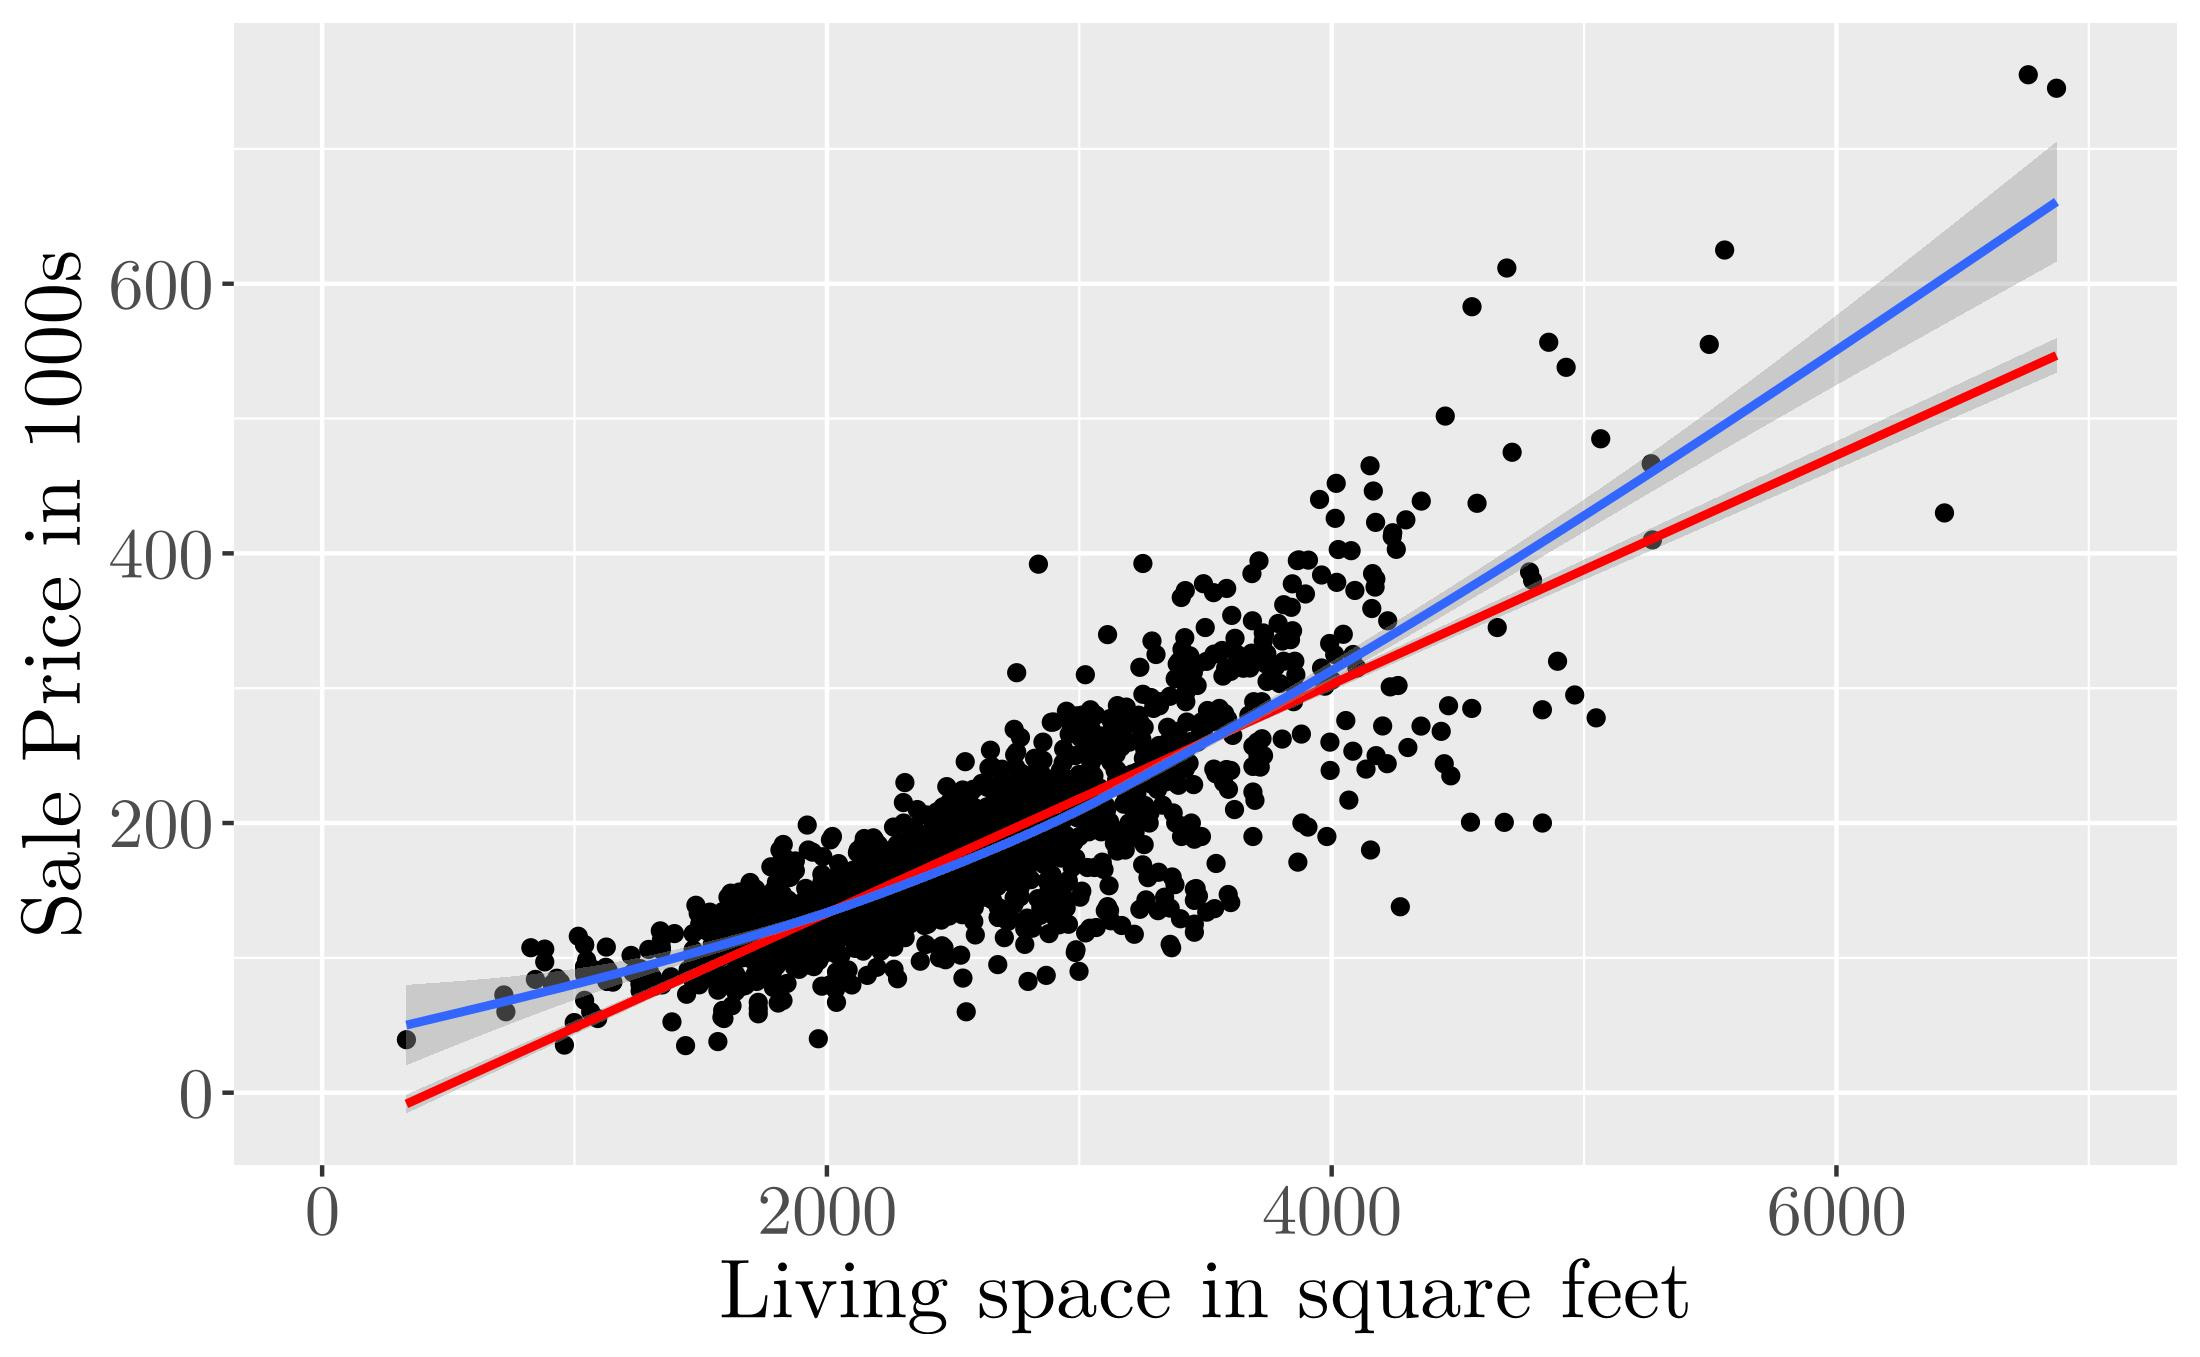
\includegraphics[width=.95\linewidth]{"/home/angelo/Documents/Uni/Courses/Advanced Statistics and programming/Assignments/assignment1/Code/h1.jpg"} 
   \caption{Total Living Space \& Sale Price}
   \label{fig:Ng2}
\end{subfigure}

\begin{subfigure}[b]{0.45\textwidth}
    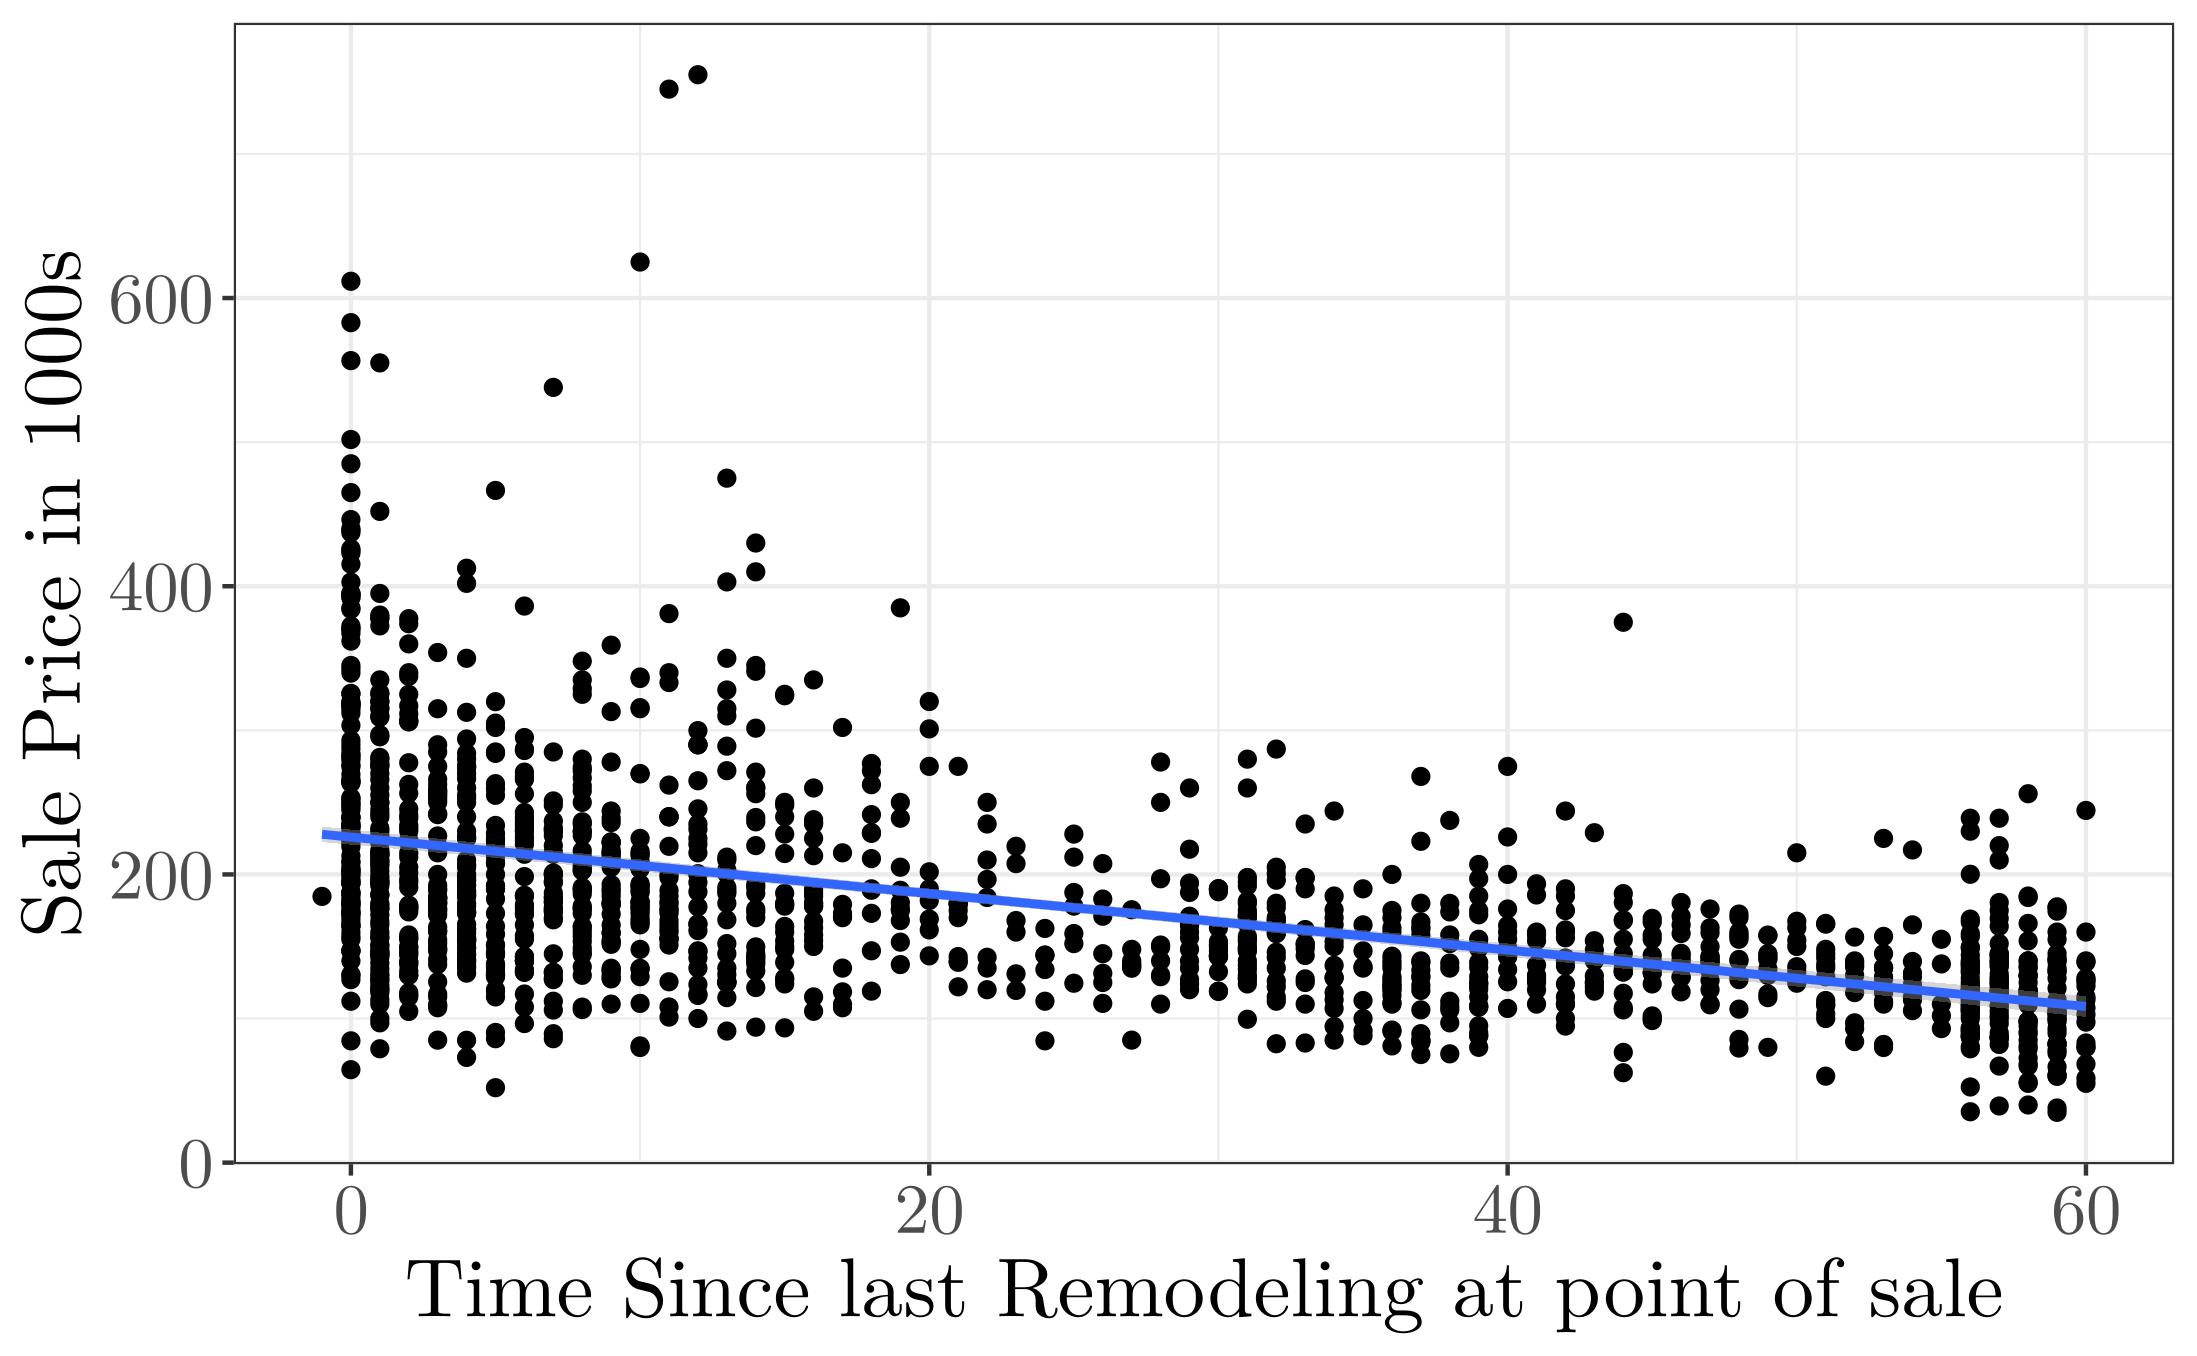
\includegraphics[width=.95\linewidth]{"/home/angelo/Documents/Uni/Courses/Advanced Statistics and programming/Assignments/assignment1/Code/h3.jpg"} 
   \caption{Time Since Remodelling \& Sale Price}
   \label{fig:Ng2}
\end{subfigure}

\begin{subfigure}[b]{0.45\textwidth}
    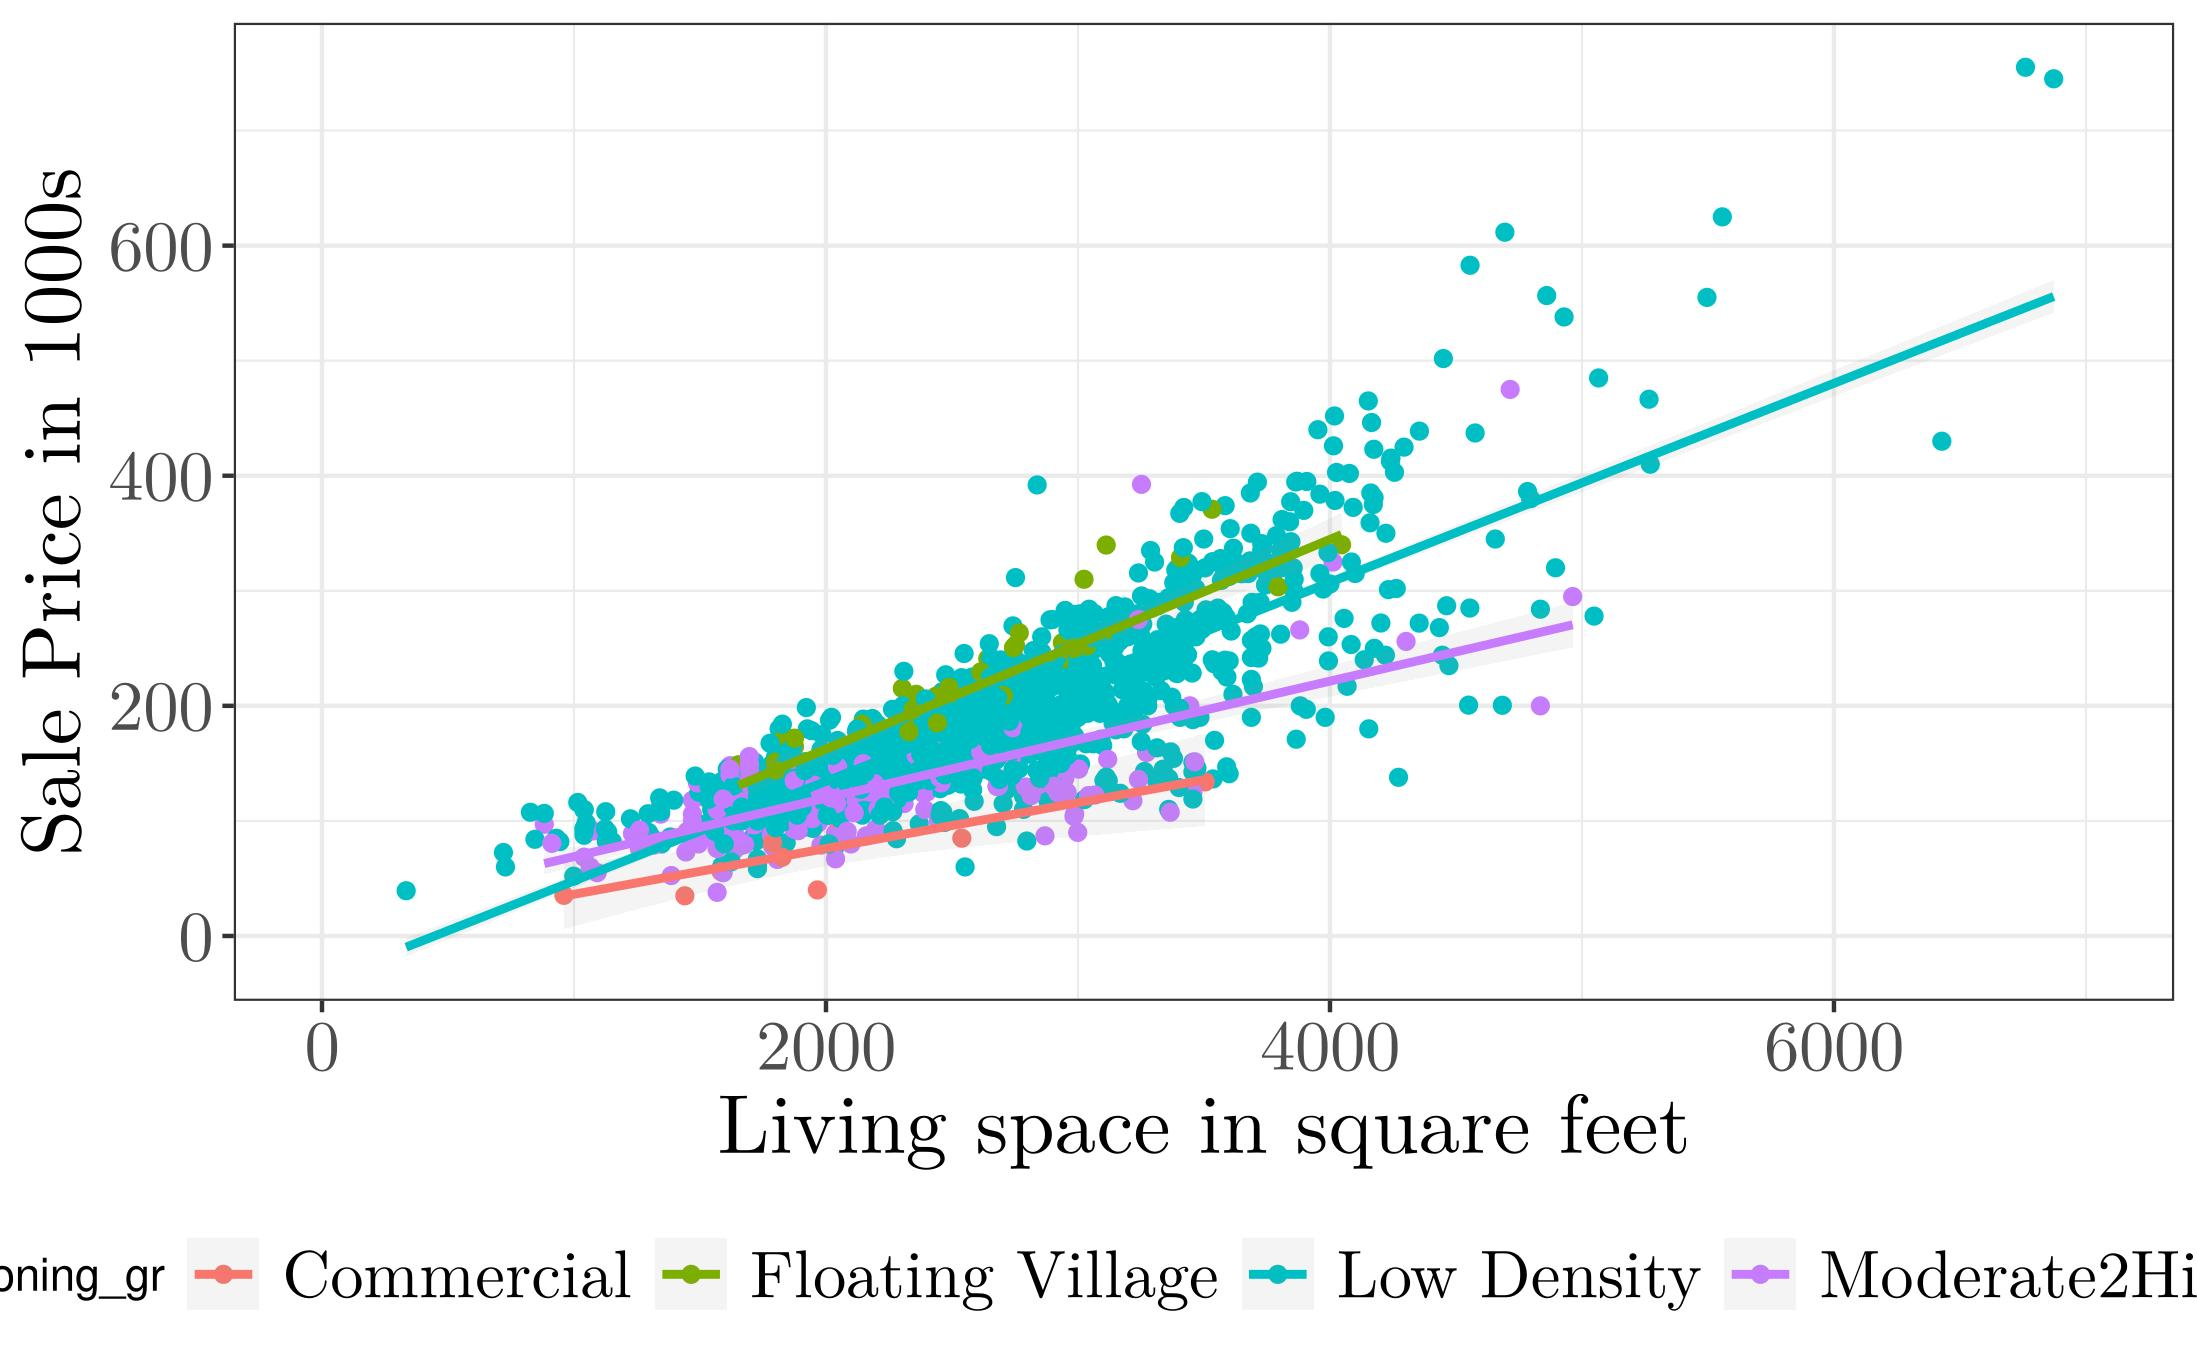
\includegraphics[width=.95\linewidth]{"/home/angelo/Documents/Uni/Courses/Advanced Statistics and programming/Assignments/assignment1/Code/h2.2.jpg"}  
   \caption{Total Living Space \& Sale Price subsectioned by Zoning}
   \label{fig:Ng2}
\end{subfigure}
\captionsetup{justification=centering}
\caption{Three Hypothesis Graphs displaying repective association with the outcome variable}
\end{wrapfigure}
For the purpose of analysing the determinants of prices of home sales in the US, the included variables in the analysis are presented in Table 1. A total of 1,460 house sales were recorded between 2006 and 2010 for the district of Ames, Iowa (USA) (Dan De Cock, 2012). As can be observed in Table 1, the mean sale price of a house was (in 1000s) \$180.921 ($SD$ = 79.443). Combined with the range [34,900, 755,000], and the median ($median$ = 163.000), a positive skewness was observed ($skew$ = 1.881), i.a. suggested by this variable being a of financial nature. The Total Living Area per property displays a mean of 2,572.89 square feet ($SD$ = 823.598, $median$ = 2479) in addition to a large range of values[334, 11,752], thereby displaying a reasonably strong positive skewness ($skew$ = 1.776).  Years Since Remodelling (at time of sale) shows that the average property did not undergo renovations for 22.95 (~23) years ($SD$ = 20.950, $median$ = 14).\footnote{This variable was constructed by deducting the Year of Sale by Year of Last Remodelling or Building Completion} This variable distributes reasonably constant across its data range, stopping out at a maximum of 60 years (See Figure 1B - quantiles). Furthermore, the variable Quality represents a rating from 1 to 10, similar to a Likert Scale. Quality has to be considered a categorical variable in this case i.a. because the distances between each rating level are not constant and the distribution is skewed (Figure 4). However, it was decided to include this variable in the table to display that certain statistics, such as the mean (= 6.099) and standard deviation (1.383) might warrant its treatment as a quantitative variable under certain assumptions. Noting this, the fact that Quality is a categorical variable will, thus, be relaxed in part 5 for demonstrative purposes. Finally, i.a. Lot Area will be used as a control variable in the regressions to control for the association larger lot sizes creating larger houses ($mean$ = 10516.830, $SD$ = 9981.265, $median$ = 9478.5). 





Additionally, multiple categorical variables are used in this assignment, such as Zoning and Year of Sale. The original (MS)Zoning variable contains seven categories, of which five contain data; these zones correspond to the administrative classification of the ground on which the properties are constructed (Commercial n = 10, Floating Village n = 65, Low-Density n = 1151, Moderate-Density n = 218, High-Density n = 16 contain data; Residential Low Density Park, Agricultural, Industrial do not contain records). For the purpose of this analysis, this number was reduced to four categories based on the similar behaviour of Moderate and High Density properties in  the data. This is interesting as Ames, Iowa, represents the stereotypical picture of a mid-western town in the US, displaying fewer densly populated areas; curtailing possibilities of extrapolation to similar samples. Thus, the main question of this analysis section focuses on the difference between Low and Medium to High density zoned properties.\footnote{Floating Village (n = 67) and Commercial (n =10) behave too differently to be merged; their sample size makes them negligbile; they are included to not rmove any data.} In addition, year of sale will be used to control for the effect of the 2008/2009 housing crisis.




Considering Figure 1a, it is notable that the positive association displayed by Sale Price and Living Area is positive and slightly increasing as one moves along the graph. This is why the most optimally fitted line is included. Finally, two outliers were exclsuded from the graph but they will be retained in the analysis further down. Figure 1b shows the negative association between Time Since Remodelling and Sale Price. Generally, the assocaition is negative, in addition to the overall distribution of the values see to be generally linear. Finally, Figure 1c shows the Total Living Space by Sale Price subsectioned by Zoning. Generally, The Low-Density Zone appears to display a stronger assocation for Living Space and Sale Price than Moderate to High. 





% Table created by stargazer v.5.2.3 by Marek Hlavac, Social Policy Institute. E-mail: marek.hlavac at gmail.com
% Date and time: Wed, Sep 14, 2022 - 15:53:27
\begin{table}[!htbp] 
\begin{adjustwidth}{-0cm}{-0cm}
\begin{threeparttable}
\small
\captionsetup{font=small, justification=raggedright,singlelinecheck=false}
\caption{\textsc{Descriptive Statistics of Numeric Varaibles}}
\centering 
  \label{}   
\begin{tabular}{@{\extracolsep{5pt}}lccccccc} 
\\[-5ex]\hline 
\hline \\[-1.8ex] 
Statistic & \multicolumn{1}{c}{Mean} & \multicolumn{1}{c}{St. Dev.} & \multicolumn{1}{c}{Min} & \multicolumn{1}{c}{Pctl(25)} & \multicolumn{1}{c}{Median} & \multicolumn{1}{c}{Pctl(75)} & \multicolumn{1}{c}{Max} \\ 
\hline \\[-1.8ex] 
SalePrice & 180.921 & 79.443 & 34.900 & 129.975 & 163.000 & 214.000 & 755.000 \\ 
Lot Area & 10,516.830 & 9,981.265 & 1,300 & 7,553.5 & 9,478.5 & 11,601.5 & 215,245 \\ 
Quality & 6.099 & 1.383 & 1 & 5 & 6 & 7 & 10 \\ 
Total Living Space & 2,572.893 & 823.598 & 334 & 2,014 & 2,479 & 3,008.5 & 11,752 \\ 
Years Since Remodeling & 22.950 & 20.641 & 0 & 4 & 14 & 41 & 60 \\ 
\hline \\[-3.5ex] 
\end{tabular} 
\begin{tablenotes}[para,flushleft]
      \small
      \item\textit{Notes:} N = 1460. Quality is technically to be considered a categorical variable
    \end{tablenotes}
\end{threeparttable}
\end{adjustwidth}
\end{table}

\section{Theoretical model and OLS assumptions}
\subsection{Hypotheses}
Based on the plots generated during the EDA, a mini theory was created to explain the variation in the sales price of properties (Figure 2). The primary parts of this theory involve Total Living Space, the corresponding Zoning of the property, and Years Since Remodelling (at point of sale). The resulting causal scheme can be seen in Figure 2 (Morgan \& Winship, 2015).

\subsubsection{Hypotheses 1}

\begin{center}
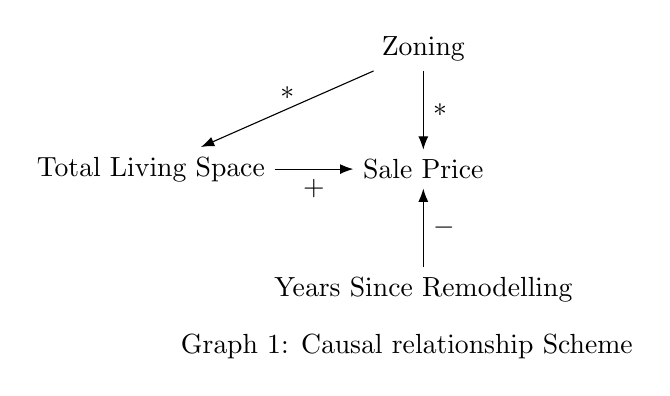
\begin{tikzpicture}
	\centering
 	\node at (3.25,-2.25) {Graph 1: Causal relationship Scheme};
    \node (1) at (0,0) {Total Living Space};
	\node (2) [right = of 1] {Sale Price};
	\node (3) [above = of 2] {Zoning};
	\node (4) [below = of 2] {Years Since Remodelling};

	\path (1) edge node[below] {$+$} (2);
	\path (3) edge node[right] {$*$} (2);
	\path (3) edge node[above] {$*$} (1);
	\path (4) edge node[right] {$-$} (2);
	

\end{tikzpicture}
\end{center}

\indent Figure 1a displays a potential direct positive association between Total Living Space (IV) and Sale Price (DV)\footnote{Including an optimally fitted line, showing potential problems of a non-linear relationship}. Thus, one expects that larger houses have a higher Sale Price. Consequently,this research asserts that:

\begin{hyp}[H\ref{hyp:first}] \label{hyp:first}
Total living space (IV) has a direct postive effect on Sales Price (DV)
\end{hyp}

\begin{center}
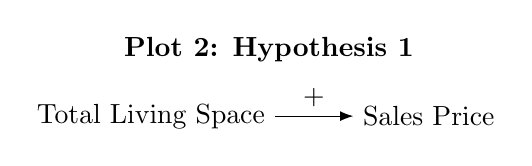
\begin{tikzpicture}
	\centering
 	\node at (1.5,0.85) {\textbf{Plot 2: Hypothesis 1}};
 	\node (1) at (0,0) {Total Living Space};
	\node (2) [right = of 1] {Sales Price};
	\path (1) edge node[above] {$+$}(2);
\end{tikzpicture}
\end{center}

\indent Subsequently, when taking the Zoning (MSZoning or MSZoning\_grouped - IV) into account to reflect the administrative borders of Ames' districts, larger houses in more densely populated areas of the city appear to have a lower price when compared to houses of same size in less densely populated areas as can be seen in Figure 1c. This suggests a separation between "down town less affluent areas" and "sub-urban affluent areas". Additionally, the effect of Total Living Area appears to be stronger for Low Density zones, which can be seen at the steeper OLS fitted line for Low Density properties when compared to Moderate-to-high density properties. Thus, the second hypothesis asserts that

\begin{hyp}[H\ref{hyp:second}] \label{hyp:second}
Zoning moderates (MIV) the direct positive association of Total Living Space (IV) and Sale Price (DV). The effect of Space and Sale Price is weaker for more (Moderate to High Low Density) densely populated areas than for rural areas (Low Density). 
\end{hyp}

\begin{center}
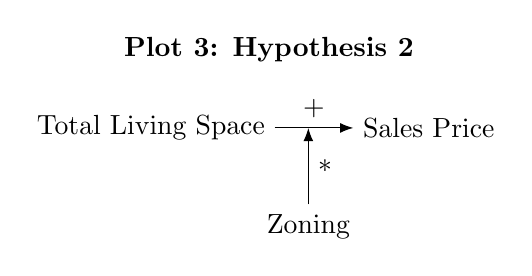
\begin{tikzpicture}
	\centering
 	\node at (1.5,1) {\textbf{Plot 3: Hypothesis 2}};
 	\node (1) at (0,0) {Total Living Space};
	\node (2) [right = of 1] {Sales Price};
	\node (3) at (2,-1.25) {Zoning};
	
	\coordinate (4) at (2,0);
	
	\path (1) edge node[above] {$+$}(2);
	\path (3) edge node[right] {$*$}(4);
\end{tikzpicture}
\end{center}

\indent Finally, Figure 1c shows that properties that are older or have not been remodelled more recently tend to have a lower sale price than newer houses. Thus, the final hypothesis asserts that Years Since Remodelling has a negative effect on Sale Price:



\begin{hyp}[H\ref{hyp:third}] \label{hyp:third}
Years Since Remodeling (IV) has a negative effect on Sale Price (DV).
\end{hyp}

\begin{center}
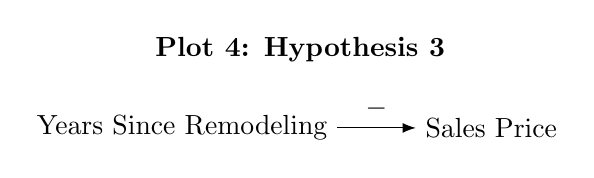
\begin{tikzpicture}
	\centering
 	\node at (1.5,1) {\textbf{Plot 4: Hypothesis 3}};
	\node (1) at (0,0) {Years Since Remodeling};
	\node (2) [right = of 1] {Sales Price};

	\path (1) edge node[above] {$-$}(2);
\end{tikzpicture}
\end{center}

The resulting population regression equation based on Graph 1 is, thus, formally expressed as:



$$ (2-1)   \\\   {SalePrice} = \alpha + \beta_{1} Total Living Area
 + \beta_{2}  Zoning - \beta_{3}  Years Since Remodeling +\epsilon$$

It is notable, that the categorical variable Zoning will be specified as a dummy variable. Additionally,  a quadratic function to address issues with non linearity Total Living Area will be used. 

\subsection{Assumptions}

\indent A1: The linearity of model parameters and error term assumption suggests that the functional form of the underlying population regression model is linear and additive. Thus, this assumption is generally assumed to hold, i.a. not having introduced quadratic or polynomial (by parameter) terms into the population regression equation (2-1). However as Figure 1b shows, there might be a quadratic, or non linear, relationship  present between Total Living Area and Sale Price. The reason why this might be the case may be that with increase values for Total Living Area, the Sale Price increases disproportionately to the linear term captured by the coefficient. This might induce reduced accuracy and goodness of fit to the model. This issue is generally rectified by e.g. a quadratic term in the regression equation of the variable in question.

\indent A2: Full rank assumes that no independent variable can be a linear function of other independent variables; thus, no optimal (or none at all) solution for the parameters in question can be found. This first part of the assumption might easily be violated when not dropping a "comparative" category of a categorical variable. However, violations of full rank might also come in the form of multicollinearity. Multicollinearity is the "almost" violation of the full rank violation as a given variable may, for instance, be highly correlated with another given variable. Primarily, standard errors of the model become unstable to the extend that inference from the model becomes impossible. Multicollinearity is almost always present with observational data (actually making regression interesting in the first place); However, the extend is more relevant. For example might be if we included the Total Living Space and the TotalNumberofRooms, both of which will be highly correlated. Further tests will be conducted to probe for this assumption violation. Solutions include the dropping (not recommended) or combining highly correlated regressors into principal components (PCA). This will be further investigated in part 4.

A3: This assumption is referred to as mean independence (or exogeneity); assuming that the error term of the model is independent of the regressors in the model. The result of the violation of A3 might result in severe consistency issues of the estimator, biasing estimates one or the other way.
A common way, this assumption is violated is are omitted variables or confounders. If a given variable is left out, part of the error term can be explained by a given variable which suffers under the influence of the confounder. For example, missing crime data by location explains why certain neighbourhoods outperform others. This is also the reason why this variable was left out of the mini theory. Thus, given a certain Neighbourhood in question, part of the variance that would have been explained by the Crime variable is now falsely attributed to Neighbourhood, biasing the estimate.

A4: The assumption of homoscedasticity assumes constant variance for the error term. However, if the variance of the estimate is varying for different observations, we face heteroscedastic variance. While this is not necessarily problematic regarding the estimated parameter (coefficient), heteroscedastictiy impacts the standard errors of the estimate, leading to problems regarding inference; (both over- and understated standard errors) potentially leading to either Type I or II error problems. In this research, this violation might occur if the e.g. sales prices vary stronger for large houses than for small houses. The resulting (averaged) standard error would neither be representatives for small and large house standard errors and, thus, inference itself. However, this assumption becomes less relevant with large samples, particularly for the estimate, as is the case here.

A5: Data generation: data can be the result of observational kind and random experiments. Due to the data originating from sales in a town in Iowa (Ames), we have to assume that the data is "fixed" to some extend (e.g. variable Quality) and random for others (eg. Sale Price itself). However, this also implies inference regarding a wider population cannot be made from this data, as it only applies to small towns in the mid-western USA. However, we can assume that the  variables collected are measured without error due to it appearing to be of an administrative source. Particularly as the sample collected can be somewhat representative of the population of small towns in the mid-western USA. 

A6: If the residuals do not follow a standard normal distribution, this might result in incorrect decisions (Type I or II; both possible). This assumption is needed for performing parametric tests and generating confidence intervals. For instance, this might be the case if we do not have a lot of observations for several subcategories (as with Neighbourhood). Subsequently, the resulting inference might be biased. However, as the sample size increases, most disturbance distributions approach the normal form. 
 Nonetheless, an indication of this assumption being violated is the presence of large amounts of outliers. As can be seen in Figure 1a (and Figure 3) the range goes from 0 to 7000 square feet, thus, omitting two extreme observations; admittedly few in numbers. Thus, we assume that this assumption is likely to hold due to the large sample size.


\section{OLS Regression and Model Fit}
\subsection{Normal Regression Results}

% Table created by stargazer v.5.2.3 by Marek Hlavac, Social Policy Institute. E-mail: marek.hlavac at gmail.com
% Date and time: Wed, Sep 14, 2022 - 15:53:27
\begin{table}[!htbp] \centering 
\begin{adjustwidth}{0.cm}{-0cm}
\begin{threeparttable}
\small
\captionsetup{font=small, justification=raggedright,singlelinecheck=false}
\caption{\textsc{Non-Robust Regression Results Part 3}}
\centering 
  \label{}
\small 
\begin{tabular}{@{\extracolsep{-2pt}}lcccccc} 
\\[-5.8ex]\hline 
\hline \\[-1.8ex] 
 & \multicolumn{6}{c}{\textit{Dependent variable:}} \\ 
\cline{2-7} 
\\[-1.8ex] & \multicolumn{2}{c}{SalePrice in 1000s} & \multicolumn{2}{c}{SalePrice in 1000s} & \multicolumn{2}{c}{ln\_SalePrice  in 1000s} \\ 
\\[-1.8ex] & Model (1) & Std. Coef.& Model (2) & Std. Coef.&  Model (3) & Std. Coef.\\ 
\hline \\[-1.8ex] 
 Constant & 15.229 &  & 24.550 &  & 3.584$^{***}$ &  \\ 
  & (25.697) &  & (24.541) &  & (0.114) & \\ 
  & & & & & & \\ 
 Living Space & 0.035$^{***}$ & 0.362$^{***}$ & 0.038$^{***}$ & 0.393$^{***}$ & 0.0003$^{***}$ & 0.684$^{***}$ \\ 
  & (0.002) & & (0.005) & & (0.00002) &  \\ 
  & & & & & & \\ 
 Years Since Remodeling & $-$0.492$^{***}$ & $-$0.128$^{***}$ & $-$0.493$^{***}$ & $-$0.128$^{***}$ & $-$0.003$^{***}$ & $-$0.170$^{***}$ \\ 
  & (0.056) &  & (0.051) &  & (0.0002) &  \\ 
  & & & & & & \\ 
 Low Dens. Zone & 16.640$^{***}$ & 0.086$^{***}$ & $-$31.118$^{***}$ & $-$0.160$^{***}$ & 0.077$^{**}$ & 0.079$^{**}$ \\ 
  & (2.753) &  & (8.368) & & (0.039) &  \\ 
  & & & & & & \\ 
 Commercial Zone & $-$25.251$^{**}$ & $-$0.026$^{**}$ & $-$35.782 & $-$0.037 & $-$0.673$^{***}$ & $-$0.139$^{***}$ \\ 
  & (11.881) &  & (35.624) &  & (0.165) &  \\ 
  & & & & & & \\ 
 Floating Zone & 18.710$^{***}$ & 0.049$^{***}$ & $-$8.247 & $-$0.021 & 0.127 & 0.065 \\ 
  & (5.258) & & (22.841) & & (0.106) &  \\ 
  & & & & & & \\ 
 Lot Area & 0.001$^{***}$ & 0.074$^{***}$ & 0.005$^{***}$ & 0.616$^{***}$ & 0.00002$^{***}$ & 0.404$^{***}$ \\ 
  & (0.0001) &  & (0.0005) &  & (0.00000) &  \\ 
  & & & & & & \\ 
  
 I(Living Space$\hat{\mkern6mu}$2) &  &  & $-$0.00000 & $-$0.002 & $-$0.00000$^{***}$ & $-$0.234$^{***}$ \\ 
  &  &  & (0.00000) &  & (0.000) &  \\ 
  & & & & & & \\ 
 Living Space:Low Dens. Zone &  &  & 0.019$^{***}$ & 0.308$^{***}$ & 0.00002 & 0.058 \\ 
  &  &  & (0.004) & & (0.00002) &  \\ 
  & & & & & & \\ 
 Living Space:Commercial Zone &  &  & 0.0001 & 0.0002 & 0.0002$^{**}$ & 0.067$^{**}$ \\ 
  &  &  & (0.017) & & (0.0001) & \\ 
  & & & & & & \\ 
 Living Space:Floating Zone &  &  & 0.013 & 0.088 & 0.00002 & 0.022 \\ 
  &  &  & (0.009) &  & (0.00004) & \\ 
  & & & & & & \\ 
 Living Space:Lot Area &  &  & $-$0.00000$^{***}$ & $-$0.647$^{***}$ & $-$0.000$^{***}$ & $-$0.396$^{***}$ \\ 
  &  &  & (0.00000) &  & (0.000) &  \\ 
  & & & & & & \\ 
  Year Sold & YES & YES & YES & YES & YES & YES \\ 
  %&  & &  &  \\ 
  % & & & & \\ 
  Overall Quality Rating & YES & YES & YES & YES & YES & YES \\  
  % & (32.730) & (32.730) & (30.513) & (30.513) \\ 
  %& & & & \\ 
  Building Type & YES & YES & YES & YES & YES & YES \\ 
  %& (2.654) & (2.654) & (2.501) & (2.501) \\ 
  % & & & & \\ 
\hline \\[-1.8ex]  
\end{tabular} 
%%%%%%%
\small 
\centering
\begin{tabular}{@{\extracolsep{39pt}}lcccccc} 
R$^{2}$ && 0.803 &   0.836 &  0.861   \\ 
Adjusted R$^{2}$ && 0.800 &  0.833 &   0.858  \\ 
Residual Std. Error && 35.548  & 32.488  & 0.150   \\ 
F Statistic& & 292.393$^{***}$    & 291.609$^{***}$   & 354.941$^{***}$    \\ 
\hline 
\hline \\[-3.5ex] 
\end{tabular} 
\begin{tablenotes}[para,flushleft]
      \small
      \item\textit{Note:} N = 1460. All observations included in any model. *** p$<$0.01, ** p$<$0.05, * p$<$0.1. Standardized regression coefficients are reported in the adjacent column to the model. For complementary regression models \textbf{see appendix}. The comparison category in "Zone" (IV) is "Moderate-to-High Density". Years in date range is 2006 to 2010. The Sale Price is represented in 1000s. 
    \end{tablenotes}
\end{threeparttable}
\end{adjustwidth}
%
\end{table}


Table 2 displays the regression results for three incrementally complex models to explain variance in Sale Price. These models were chosen as they concisely combine most necessary information for part 3 and 4. Standardized coefficients are reported adjacent to their respective models. Standard errors are not robust (see part 4). 
Overall, all three reported models are each jointly significant, displaying a significant F-test ($F$ = 292.393, $p$ $<$  0.001; $F$ = 291.609, $p$ $<$ 0.001, $F$ = 354.941, $p$ $<$  0.001). 
Not considering the control variables and interaction terms, the results of model (1) suggest that Total Living Area has a significant positive effect on Sale Price ($\hat{\beta}$ = 0.035, $p$ < 0.001), thus, finding support for hypothesis 1. Therefore, an increase in Living Area by one square feet increases the sale price by \$35\footnote{remember: Sale Price is in 1000s}.
Additionally, Years Since Remodelling follows the expected pattern and shows a significant negative effect on Sale Price ($\hat{\beta}$ = -0.492, $p$ $<$ 0.001). Moreover, when compared to the Moderate to High Zoning, the Low Density Zone shows a significantly higher Sale Price(s) of \$16,640 ($\hat{\beta}$ = 0.086, $p$ $<$ 0.001).

\indent Now considering model (2), which includes several interaction terms and one quadratic term.\footnote{Note: model (3) will be used in part 4} We see that the coefficients for Living Space ($\hat{\beta}$ = 0.038, $p$ $<$ 0.001) and Years Since Remodelling ($\hat{\beta}$ = -0.493, $p$ $<$ 0.001) remain similar to those in model (1). Furthermore, regarding the interaction terms, the Low Density Zone seems to display a stronger positive relationship in terms of Living Space and Sale Price than the Moderate to High density zone, by \$19 more per square foot ($\hat{\beta}$ = 0.019, $p$ $<$ 0.001). Furthermore, the quadratic term of Living Space is significant, suggesting an increase of Sale Price beyond what the linear term captures ($\hat{\beta}$ = -0.002, $p$ $<$ 0.01). However, what is most striking about the model is that the Low Density Zone appears to change its direction in model (2); when compared to the Moderate to High Density Zone, the Low Density Zone reports a lower Sale Price of around \$31118 ($\hat{\beta}$ = 31.118, $p$ $<$ 0.001). It might be noted, that this might be explained by the aforementioned interaction effect of Living Space and Low Density Zone (see next subsection).

Finally, addressing the fact that the inclusion of new variables and interaction terms always increases the explained variance in the outcome; reported in $R²$. Thus, to control for this fact the $adj.R²$ corrects for the addition of a new variable(s) only improving the model by chance.
Thus, as reported in Table 2, model (1) explains 80.3\% ($R²$) of the variance in Sale Price. Model (2) explains 83.6\%. This was to be expected due to the new terms. Consequently, the $adj.R²$ of model (2) is 0.833, which is higher than the reported $adj.R²$ in model (1), which suggests that the inclusion of the interaction terms (and quadratic terms) improved upon the model and its fit on the data. 



\subsection{Standardized coeffiicents}
However, while the evaluation of the fit of the models can be done via $adjR²$, the comparisons of the regressors is not directly possible. This is due to the difference in ranges for the data for each variable. Subsequently, Table 2 reports the standardized coefficients adjacent to the unstandardised coefficients. Overall, when ignoring the control variable (model (2)) Lot Area ($\hat{\beta}std$ = 0.616, $p$ $<$ 0.001), of the theory relevant variables, it might appear that Living Space displays the largest effect Size ($\hat{\beta}std$ = -0.393, $p$ $<$ 0.001). This is also in accordance with model (1). However, because of this specific reason, the control variable Lot area, and its interaction with Living Space, was included, as it displays a very large standardized negative term ($\hat{\beta}std$ = -0.647, $p$ $<$ 0.001). Thus, while it might appear from the standardized coefficients that Living Space has the largest effect size, it is notable that this effect is counterbalanced by the large interaction effect of Lot Area and Living Space. Thus, it is notable that Years Since Remodelling ($\hat{\beta}adj$ = -0.128, $p$ $<$ 0.001) is still comparatively large. Consequently, among the quantitative relevant variables, the largest effect size should be attributed to Years Since Remodelling because of the net effect of the interaction effect of Living Space in the subgroup of Low Density Zones being of an opposite direction when compared to Moderate to High Density Houses. Finally, due to the standardized coefficient for the interaction of Living Space and Low Density Zone $\hat{\beta}adj$ = 0.308, $p$ $<$ 0.001) now exceeding the negative std. coefficient for Low Density Zone $\hat{\beta}adj$ = -0.160, $p$ $<$ 0.001), this suggests some support for hypothesis (2) after all.
\indent Thus, in model (2) the largest effect size belongs to the interaction term of Living Space and Lot area. However, considering only single variables (without controls), the larges effect size is technically the Living Space and Lot Area interaction, with the caveat that Years Since Remodelling is still quite large in addition to Living Space coefficient pointing into the other direction. \footnote{Please note that the interpretation of effect sizes follows that if eg. X changes by one standard deviation, how many standard deviations does Y change. This is uninformative, and, thus, is not reported}



\section{Diagnostic checking}
\subsection{Assumption 1}
As can be seen in Figure 1a, Total Living Space tends to display non linearity with the outcome. Subsequently, Table 2 shows the inclusion of a quadratic term when comparing Model 2 and 3. Overall, including not only the quadratic term ($\hat{\beta}$ = 0.002, $p$ $<$ 0.001; $adj.\hat{\beta}$ = 0.234, $p$ $<$ 0.001), but also log scaling the outcome improves the model beyond chance.\footnote{log scaling is applied because of the financial nature of Sale Price, which is commonly transformed using log} Thus, the issue of non-linearity is reduced. however, the inclusion of the log specification also increases the difficulty in interpreting the results. This is why model (2) in Table 2 can be used as a somewhat comparable model. 

\subsection{Assumption 2}
\begin{wraptable}{L}{8.5cm}

\begin{threeparttable}
\small
\captionsetup{font=small, justification=raggedright,singlelinecheck=false}
\caption{\textsc{VIF reports }}
\centering 
  \label{}
\small 
\begin{tabular}{@{\extracolsep{-7pt}}lcccccc} 
\\[-5.8ex]\hline 

 & GVIF & Df & GVIF$\hat{\mkern6mu}$(1/(2\textasteriskcentered Df)) \\ 
\hline \\[-1.8ex] 
tot\_liv\_area & $22.682$ & $1$ & $4.763$ \\ 
y\_since\_rem & $1.535$ & $1$ & $1.239$ \\ 
low\_density\_zone & $16.161$ & $1$ & $4.020$ \\ 
commercial\_zone & $11.942$ & $1$ & $3.456$ \\ 
floating\_zone & $30.700$ & $1$ & $5.541$ \\ 
I(tot\_liv\_area$\hat{\mkern6mu}$2) & $31.756$ & $1$ & $5.635$ \\ 
LotArea & $32.949$ & $1$ & $5.740$ \\ 
YrSold & $1.051$ & $4$ & $1.006$ \\ 
OverallQual\_cat & $4.301$ & $9$ & $1.084$ \\ 
Building\_type & $1.189$ & $1$ & $1.090$ \\ 
tot\_liv\_area:low\_density\_zone & $31.262$ & $1$ & $5.591$ \\ 
tot\_liv\_area:commercial\_zone & $11.544$ & $1$ & $3.398$ \\ 
tot\_liv\_area:floating\_zone & $31.772$ & $1$ & $5.637$ \\ 
tot\_liv\_area:LotArea & $46.292$ & $1$ & $6.804$ \\ 
 
\hline \\[-3.5ex] 
\end{tabular} 



\begin{tablenotes}[para,flushleft]
      \small
      \item\textit{Note:} N = 1460. 
    \end{tablenotes}
\end{threeparttable}

%
\end{wraptable}

Considering multicollinearity, Table 3 reports the VIF for the variables in the main model (3) (see Table 2) excluding control-categorical variables. In order to assess multicollinearity, the VIF was calculated. To make the resulting VIF comparable, the GVIF\^(1/(2*Df)) is used(Fox \& Monette, 1992). While some variables display a VIF of more than 5, this does not automatically suggest multicollinearity. However, this necessitates further analysis. Considering i.a. Table 2 again, one can see that the standard errors remain stable across all models\footnote{(not reported) There seems to be some multicollinearity problems with the control variable categories of Quality, which is to be expected due to it being a rating variable with sometimes very similar categories}. The inclusion of more variables, interaction terms, or scaling the outcome, does not cause the standard error estimates to vary considerably beyond what can be expected. The only caveat observed in Part 3 was the change in sign by the Low Density Zone, which might be explained by its positive interaction term with Living Space. Finally, the stability of the model and the significance of most of the terms in context of the significance of the overall model ($F$ = 354.941, $df$ = 25) indicates that multicollinearity might not pose a considerable problem in this model (2).


\subsection{Assumption 4}
Table 4 presents the regression results for model (3) from Table 2 with robust standard errors (White) in model (2) of Table 4, and clustered standard errors by Neighbourhood in model (3). Neighbourhood was chosen due to the assumption that houses in the same neighbourhood might share variance (such as lower crime neighbourhoods). Overall, this research does not seem to suffer from any systematic problems of heteroscedasitity, considering the stability of the standard errors across all three reported model in Table 4.\footnote{Large Changes in Standard errors in the Commercial Zone category and Floating Zone category might be attributable to their very small sample size}. Further, the residuals vs fitted plot in Figure 2, in addition to the Breusch Pagan test ($BP$ = 106.62, df = 25, $p$ < 0.001) lending support to reject a non-normal distributed residuals hypothesis, suggest that heteroscedasticity does not seem to pose a problem in this model. 


% FIGURE 

\begin{wrapfigure}{L}{11.5cm}
		\centering
         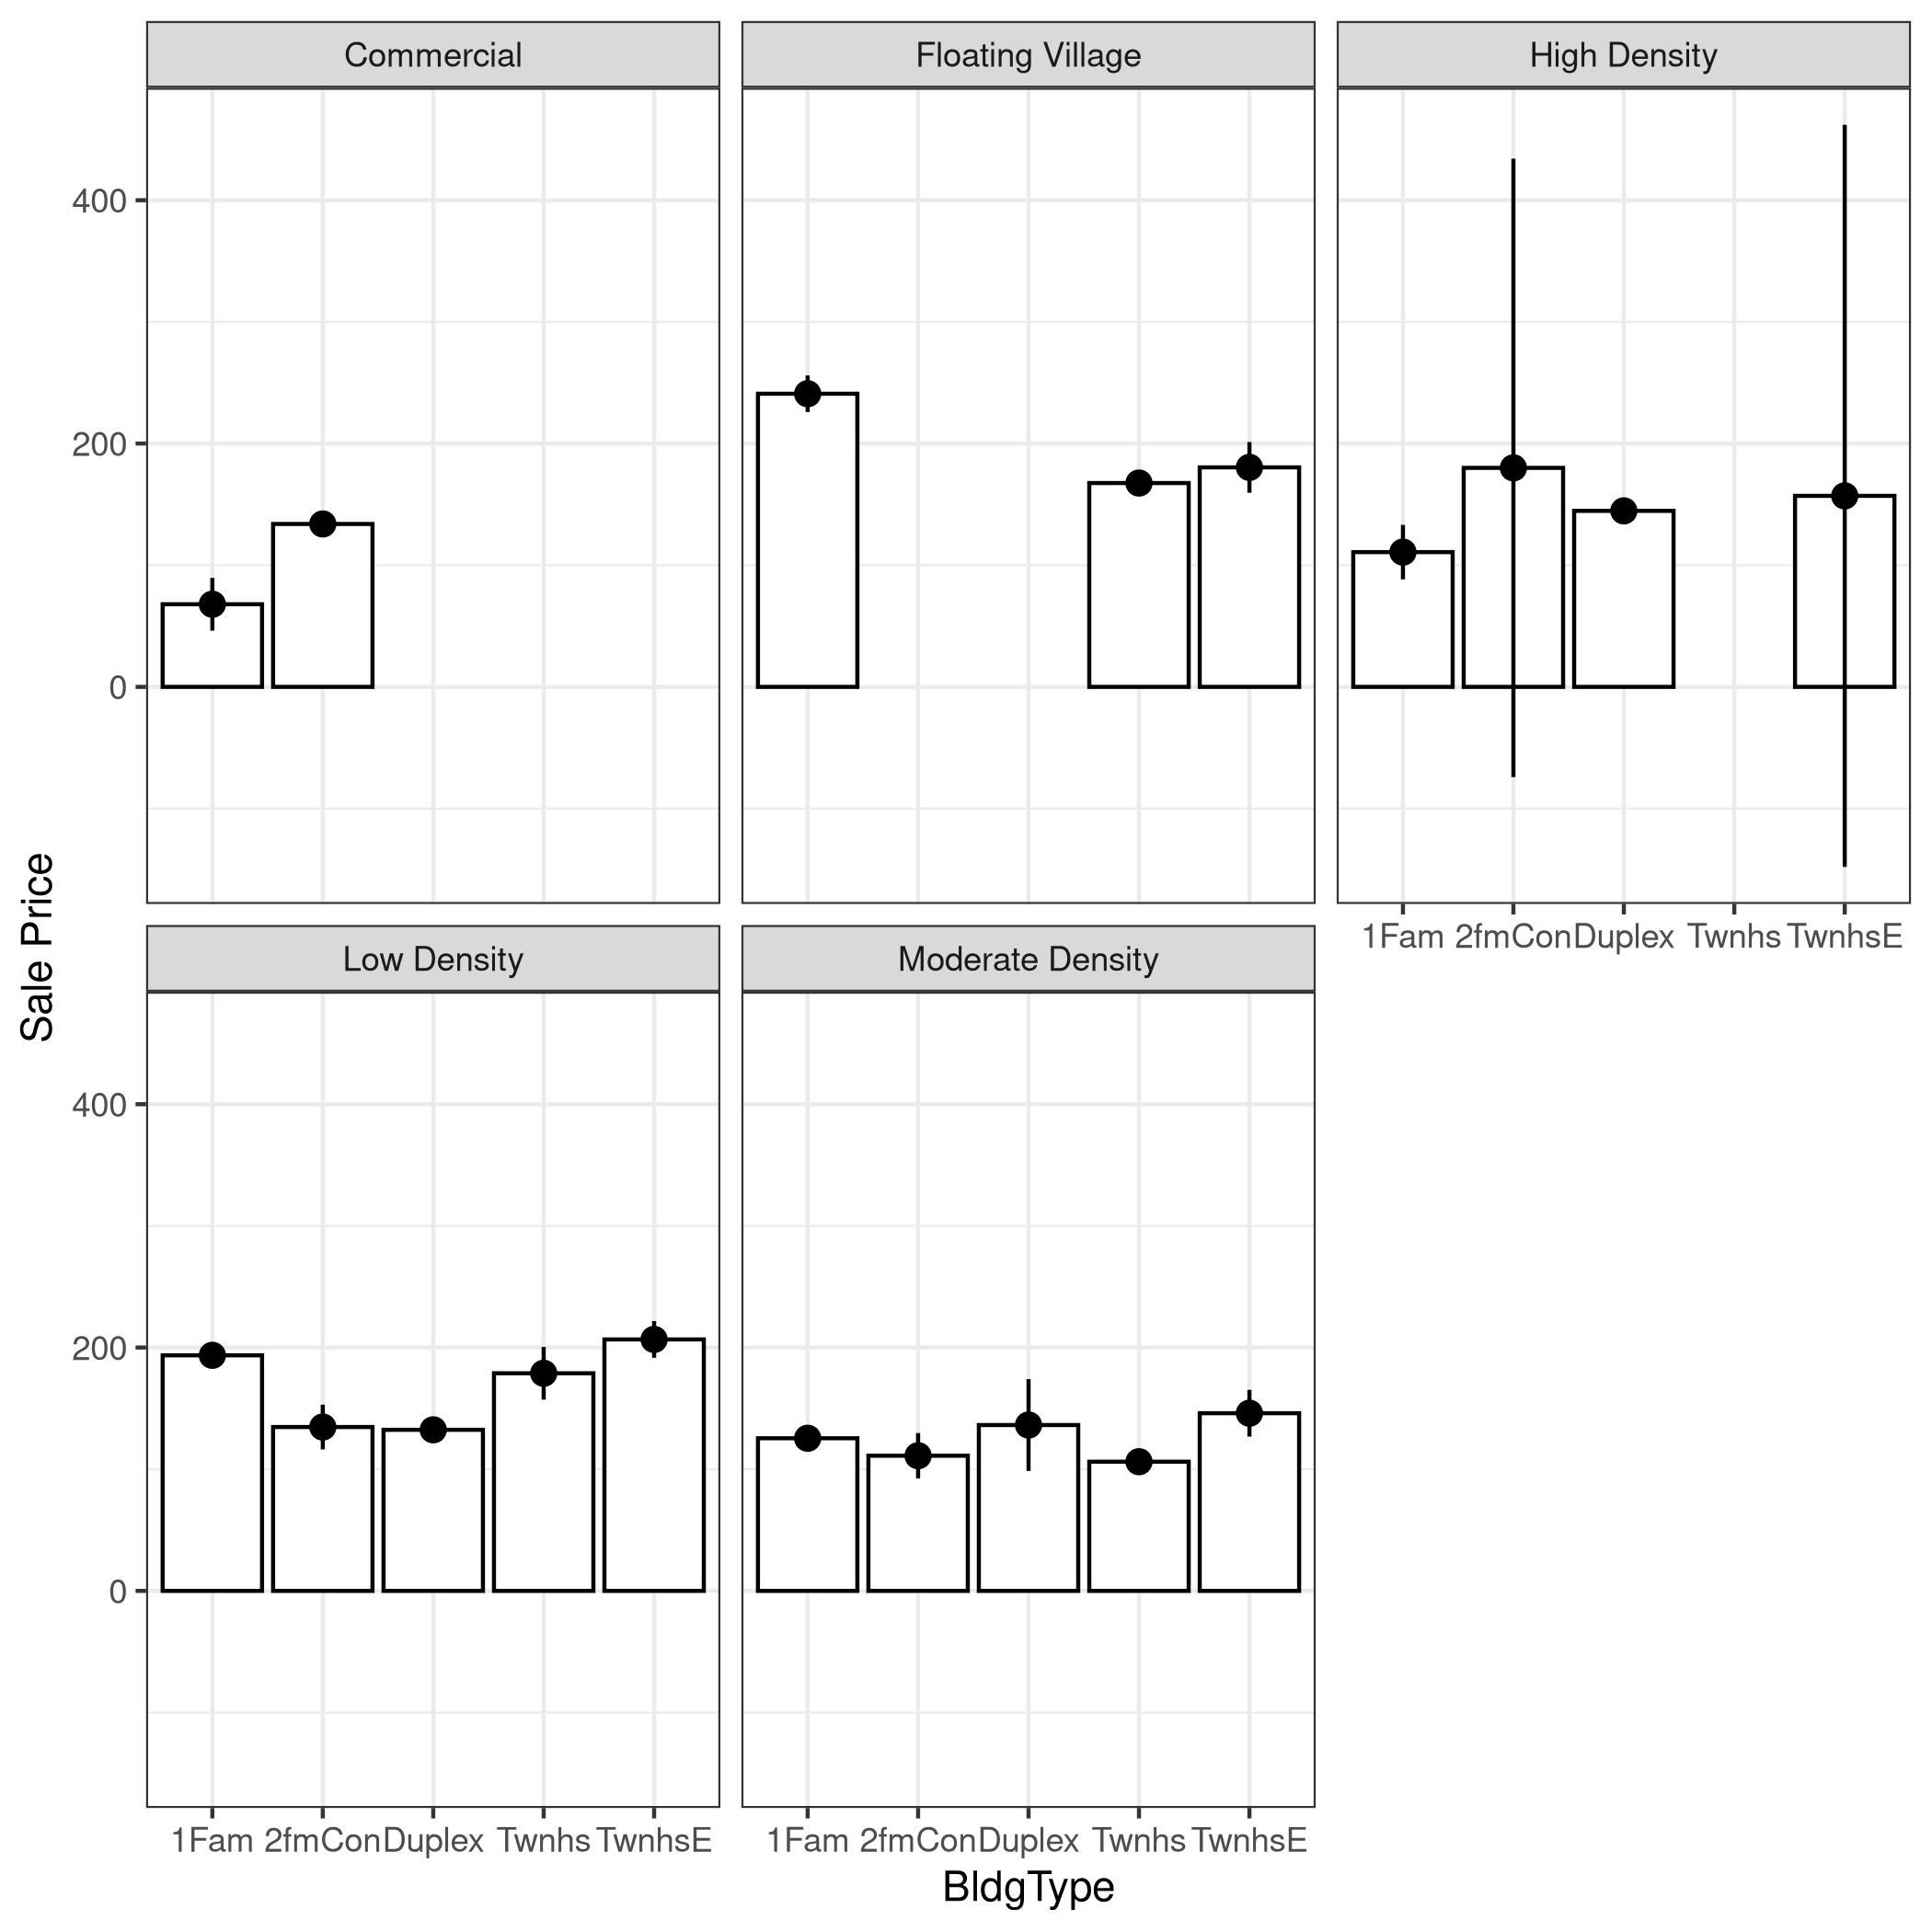
\includegraphics[scale=0.4]{"/home/angelo/Documents/Uni/Courses/Advanced Statistics and programming/Assignments/assignment1/Code/normalityplots.png"}
         \small
         \caption{Residual Distribution Plots}
\end{wrapfigure}




\subsection{Assumption 6}
Considering the $N=$ 1460 sample size, applying the Shapiro-Wilk test returns an expected rejection of non-normal distribution of the residuals ($SW$ = 0.95161,  $p$ $<$ 0.001). Interestingly, without log scaling the Sale Price (DV) and introducing the quadratic term for Total Living Space, the normality plot in Figure 3 suggests some non-linearity, while still showing a significant Shapiro-Wilk test ($SW$ = 0.8712,  $p$ $<$ 0.001). However, this largely disappears after applying both the log scale on the outcome and the quadratic term on the Total Living Space in model (3) of Table 2 (see Figure 2 upper right). Nevertheless, due to the large sample size, issues with the normal distribution assumption of the residuals can be neglected in this case. 
% FIGURE 
\begin{figure}
		\centering
         \includegraphics[scale=0.20]{"/home/angelo/Documents/Uni/Courses/Advanced Statistics and programming/Assignments/assignment1/Code/BIGNONNORMALITYPROBLEMWITHOUTLOGSCALE"}
         \small
         \caption{Normality Plots}
\end{figure}

% FIGURE 
\begin{figure}
		\centering
         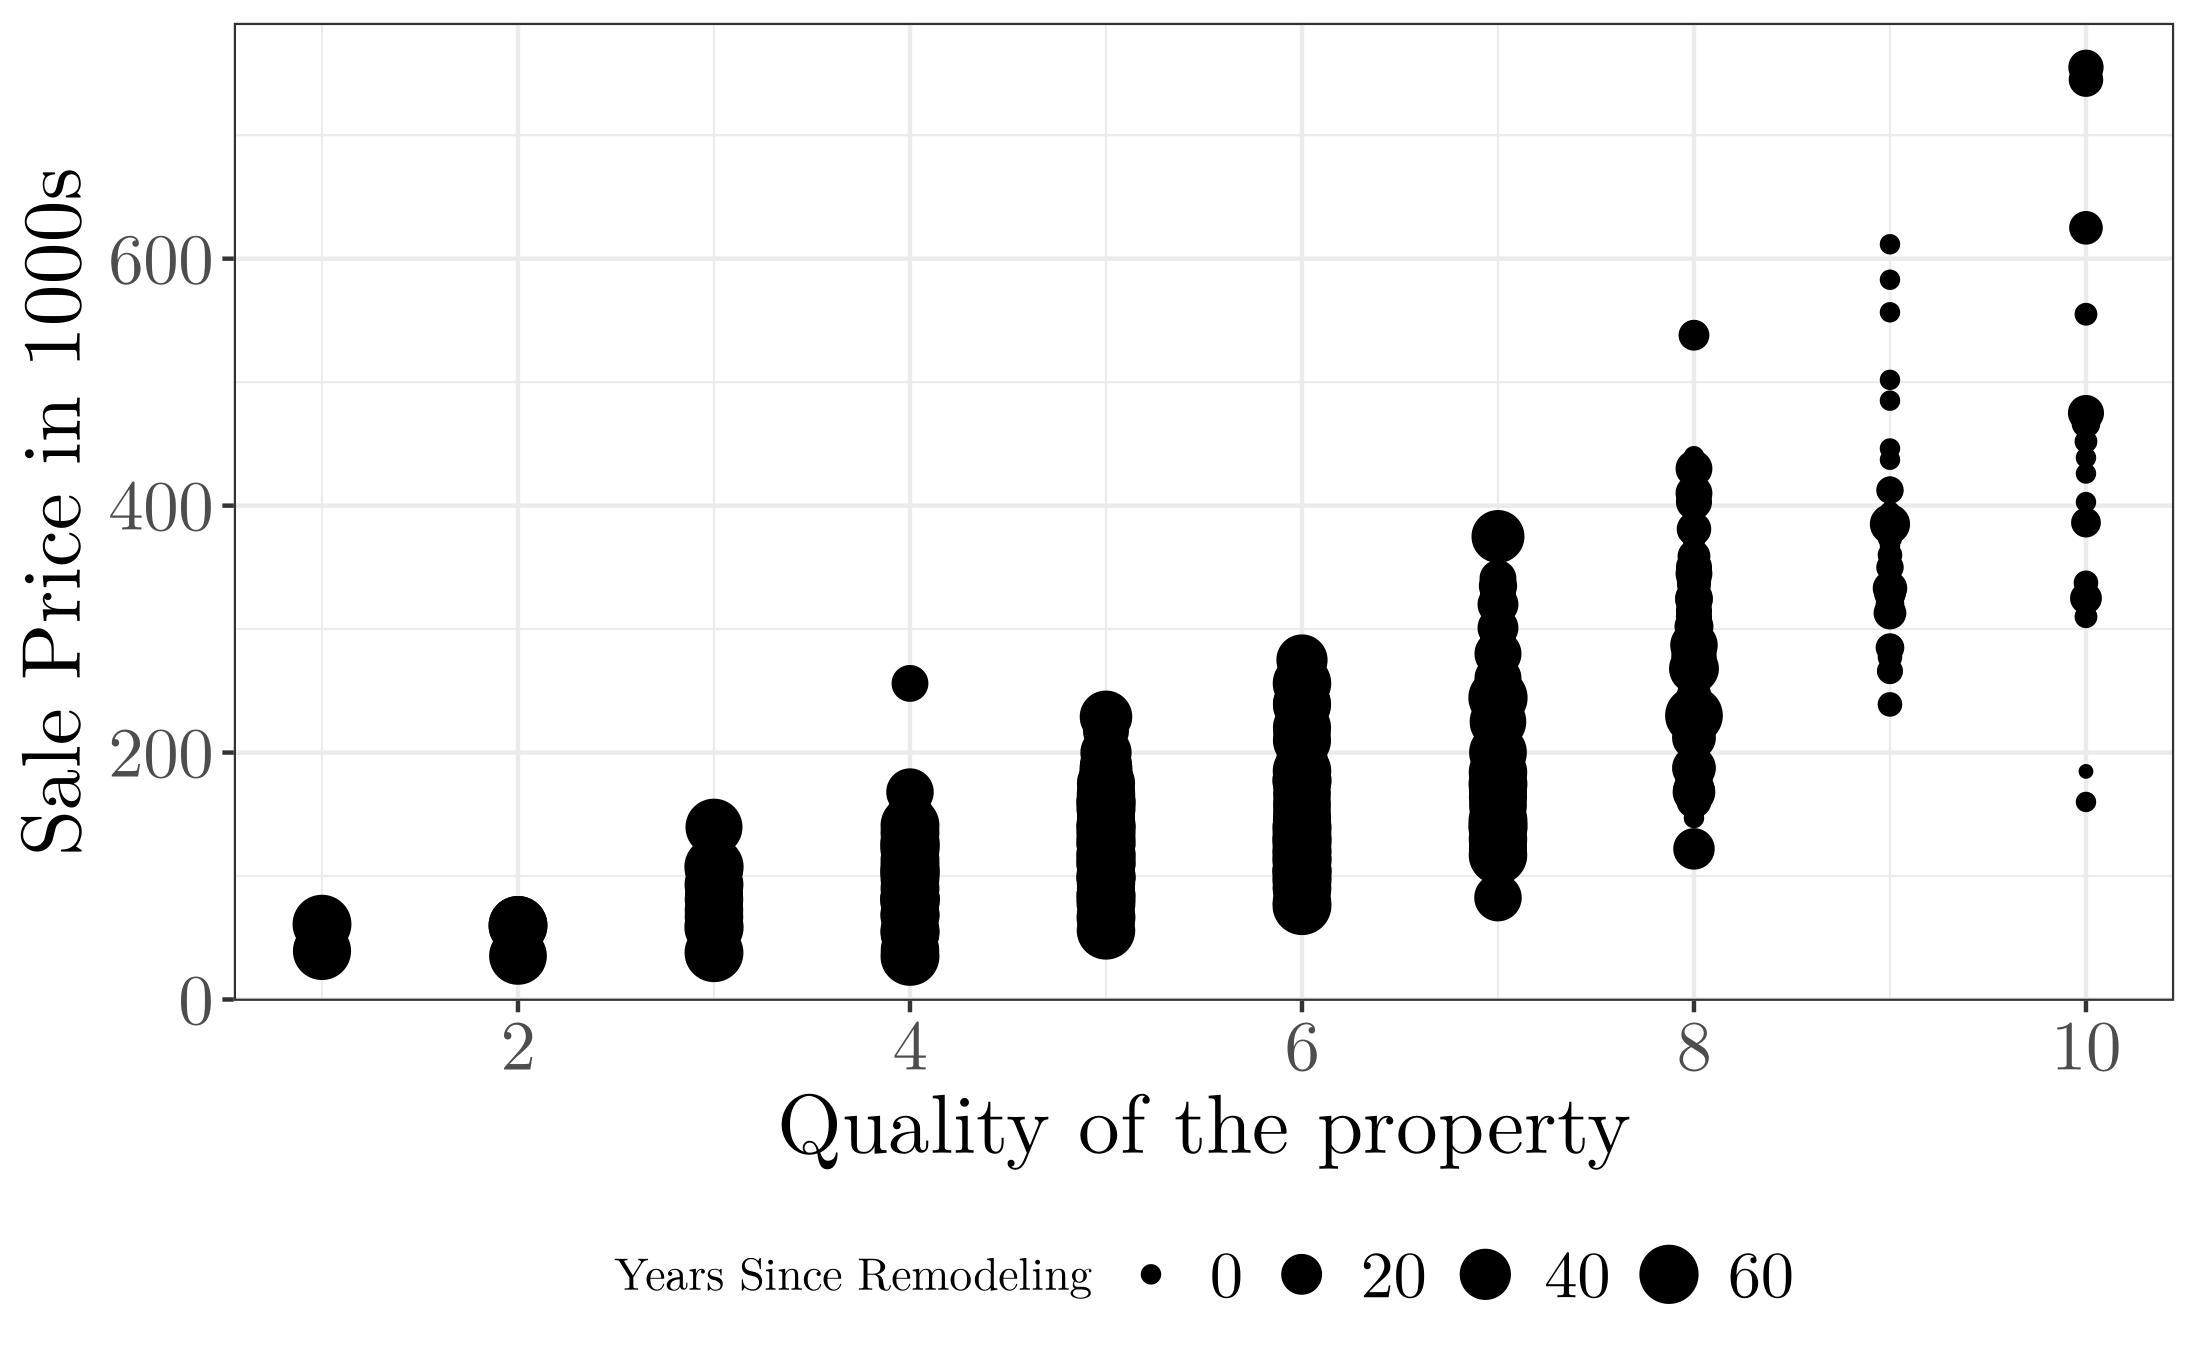
\includegraphics[scale=0.4]{"/home/angelo/Documents/Uni/Courses/Advanced Statistics and programming/Assignments/assignment1/Code/supplement_appendix_Quality_yearssinceremodeling_sale.jpg"}
         \small
         \captionsetup{justification=centering,margin=0cm}
         \caption{Quality of Property to Sales moderated by Years Since Remodelling}
\end{figure}


\section{Subset analyses}
Finally, the subset analysis considers two different models due to brevity concerns. For sake of this exercise, Quality will be considered a quantitative variable. additionally, assumptions regarding normality and scaling are ignored for simplicity. The preceeding models show the interaction on Building type, Quality and Years Since Remodelling. 
As can be seen in Table 5, the subset analysis contains two types: the interaction of Years Since Remodelled and Overall Quality, both of a quantitative nature (see Figure 4), and Zoning, where the categories of interest are Low Density vs High Density (see Figure 1c). Interestingly, Figure 4 shows that High Quality houses tend to be newer; this is why we will analyse this now.
From the interpretation of Quality ($SW$ = 31.370  $p$ $<$ 0.001) and Years Since Remodelling ($SW$ = 1.890,  $p$ $<$ 0.001) as an interaction term ($SW$ = -0.418,  $p$ $<$ 0.001) follows, as expected, that for one year more not remodelled, the effect of a unit change in Quality on Sale Price is reduced by \$418. Thus, Years Since Remodelling has a negative (assumed) effect on the relationship of Quality on Sale Price. 
Following this line of thought, as was done in Part 3, the interpretation of subset analysis regarding simple categories is that Low Density Zone properties show a \$1670 lower Sale Price than Moderate to High Density properties. Then, considering the interaction term of Living Area and Low Density Zone, this implies that given the Zone Low Density, the effect of Living Area on Sale Price is \$ 9 stronger per additional square feet in Living Area when compared to Moderate to High Density Zone. If we were to analyse for instance the category of Floating Zone interacting with Total Living Area again only compares to the Moderate to High Zone; for different comparisons, other models with different comparison groups would have to be run.\footnote{Please note again, that the groups of Commercial and Floating are ignored in this analysis as their categories are contain few observations}

% FIGURE 
\begin{figure}[htp]
\begin{adjustwidth}{-2.5cm}{-2.5cm}
		\centering
         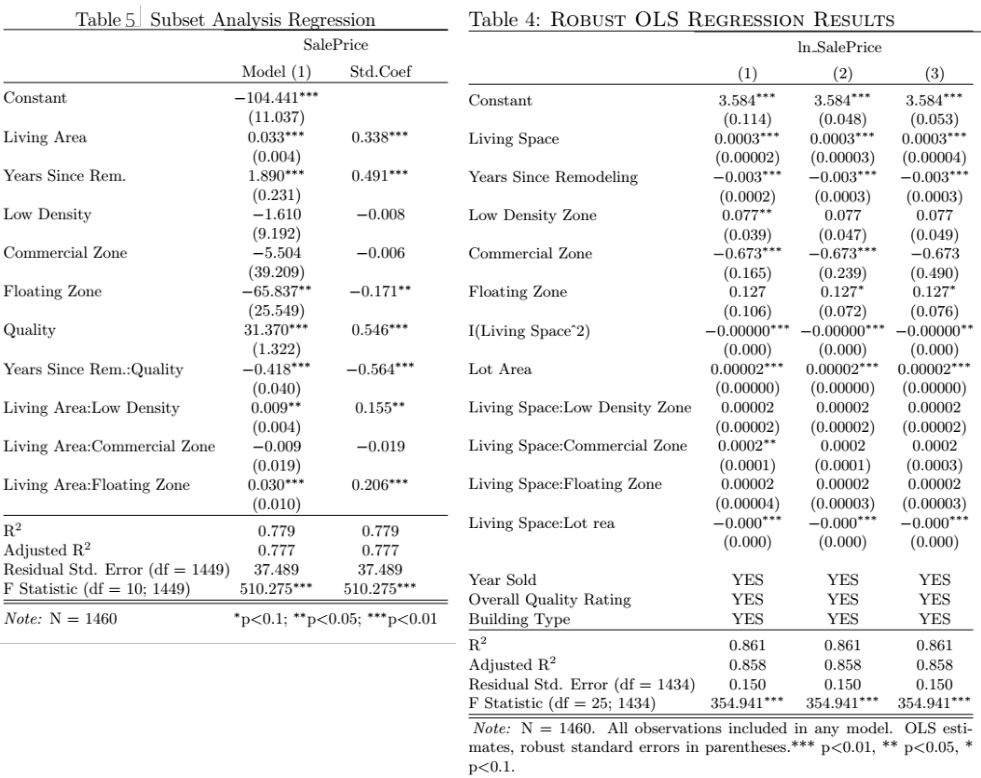
\includegraphics[scale=0.55]{"/home/angelo/Documents/Uni/Courses/Advanced Statistics and programming/Assignments/assignment1/Code/IMPORTANT2.png"}
         \small
\end{adjustwidth}
\end{figure}




















\newpage
\newpage
\section{Citations}
\indent \indent Causal Graphs in LaTex - Daniel Kumor. (2018, August 15). Retrieved September 16, 2022, from $https://dkumor.com/posts/technical/2018/08/15/causal-tikz/$

\indent Fox, J., \& Monette, G. (1992). Generalized collinearity diagnostics. $Journal of the American Statistical Association, 87(417)$, 178-183.

\indent Hlavac, M. (2018). $stargazer: Well-Formatted Regression and Summary Statistics Tables.$ Central European Labour Studies Institute (CELSI). https://CRAN.R-project.org/package=stargazer

\indent $Housing Prices Competition for Kaggle Learn Users, Dean De Cock$. (n.d.). Retrieved September 14, 2022, from https://www.kaggle.com/c/home-data-for-ml-course/data?select=train.csv

\indent Morgan, S. L., \& Winship, C. (2015). $Counterfactuals and causal inference.$ Cambridge University Press.


\indent  R Core Team (2013). R: A language and environment for statistical
  computing. R Foundation for Statistical Computing, Vienna, Austria.
  URL http://www.R-project.org/.
  
\indent Wickham H, Averick M, Bryan J, Chang W, McGowan LD, François R, Grolemund G, Hayes A, Henry L, Hester J, Kuhn M, Pedersen TL, Miller E, Bache SM, Müller K, Ooms J, Robinson D, Seidel DP, Spinu V, Takahashi K, Vaughan D, Wilke C, Woo K, Yutani H (2019). “Welcome to the tidyverse.” $Journal of Open Source Software$, 4(43), 1686. $doi:10.21105/joss.01686.$

Wickham H (2007). “Reshaping Data with the reshape Package.” $Journal of Statistical Software$, 21(12), 1–20. http://www.jstatsoft.org/v21/i12/.





\newpage
\newpage


\begin{lstlisting}[language=R]
# clear environment
rm(list=ls())

# import the necessary libraries
library("tidyverse")
library("stargazer")
library("tidyverse")
library("reshape")
library("Hmisc")
library("ggplot2")
library("dplyr")
library("moments")
library ("lm.beta")
library("fastDummies")
library("AER")
library("DAAG")
loadfonts()




setwd("/home/angelo/Documents/Uni/Courses/Advanced Statistics and programming/Assignments/assignment1")

df <- read.csv("Data/train.csv", header= TRUE, sep= ",")



# display missing values by column
colSums(is.na(df))

# select all columns which have missing data 
which(colSums(is.na(df))>0)









df_ <- df[, c(
  'Id',
  'SalePrice',
  'MoSold',
  'YrSold',
  'YearRemodAdd',
  'LotArea',
  'GrLivArea',
  'TotalBsmtSF',
  'BldgType',
  'MSZoning',
  'Neighborhood',
  'OverallQual'
)]


# create the interesting varaibles
df_$tot_liv_area <- df_$GrLivArea + df_$TotalBsmtSF

# time since remodeling at year of sale in years
df_$y_since_rem <- df_$YrSold - df_$YearRemodAdd



# adjust for family homes
# the distinction made here is simply that:
# stand alone house vs multiple houses together
match_df = data.frame(
  old = c("1Fam", "2fmCon", "Duplex",  "Twnhs", "TwnhsE"),
  new = c(
    "Single Family Home",
    "Multi-Unit Homes",
    "Multi-Unit Homes",
    "Multi-Unit Homes",
    "Multi-Unit Homes"
  )
)

df_ <-
  df_ %>% mutate(Building_type = match_df$new[match(BldgType, match_df$old)])



# group zoning
#' I have decided to leave the groups as small groups sizes are only a problem for anova
#' https://stats.stackexchange.com/questions/219071/sample-size-of-the-levels-of-a-categorical-variables -- CITE!
#' https://journals.plos.org/plosone/article?id=10.1371/journal.pone.0229345
#' Additionally: the plot shows that even if these groups are small, they do not scatter that much
match_df = data.frame(
  old = c("C (all)", "FV", "RH", "RL", "RM"),
  new = c(
    "Commercial",
    "Floating Village",
    "High Density",
    "Low Density",
    "Moderate Density"
  )
)

df_ <-
  df_ %>% mutate(MSZoning = match_df$new[match(MSZoning, match_df$old)])

#' however, further analysis will show that these two groups are quite comparable; so for the purpose of this analysis they are merged as well
#' Commercial and FV are too different to even be considered merged
match_df = data.frame(
  old = c("Commercial", "Floating Village", "High Density", "Low Density", "Moderate Density"),
  new = c(
    "Commercial",
    "Floating Village",
    "Moderate2High Density",
    "Low Density",
    "Moderate2High Density"
  )
)

df_ <-
  df_ %>% mutate(MSZoning_gr = match_df$new[match(MSZoning, match_df$old)])

# fix y_since_rem
df[df$y_since_rem < 0, "y_since_rem"] <- 0








table_out <- table(df_$OverallQual_cat )
#Add cumFreq and proportions
table_out <- transform(table_out, cumFreq = cumsum(Freq), relative = prop.table(Freq))

#' based on the resulting table, the Quality variables will be split into 
#' 3 groups; these groups will not be equally distributed, however, the size of the underlyign groups tend to be somewhat simialr
#' Furthermore: one would expect that about 67% of respondents are in the one std region 
#' Thus, we assume that the distribution somewhat is according that of a normal distributi
table_out$cumsum_freq <- cumsum(table_out$relative)
table_out


match_df = data.frame(
  old = c( 1,2,3,4,5,6,7,8,9, 10),
  new = c(
    "Low",
    "Low",
    "Low",
    "Low",
    "Medium",
    "Medium",
    "Medium",
    "High",
    "High",
    "High"
  )
)

df_ <-
  df_ %>% mutate(OverallQual_grouped = match_df$new[match(OverallQual, match_df$old)])



# adjust the scale of saleprice for easier handling
df_$SalePrice <- df_$SalePrice / 1000

# to make it clear that only certain operations can be performed on the data
# ID should be a character as string/factor operations are resptrictive by design
# i.e. no mathematical operations
df_$Id <- as.character(df_$Id)

# The month sold shoul also be considered a factor for the same reason before
df_$MoSold <- as.factor(df_$MoSold)
df_$YrSold <- as.factor(df_$YrSold)

# these are just standard variables to be converted to factors
df_$Neighborhood <- as.factor(df_$Neighborhood)
df_$BldgType <- as.factor(df_$BldgType)
df_$MSZoning <- as.factor(df_$MSZoning)

# OverallQual can be interpreted as both categorical and numeric; It wil be further elaobrated upon
df_$OverallQual_cat <- as.factor(df_$OverallQual)


# drop some columns which are now no logner needed
df_ = df_[, !(names(df_) %in% c("YearRemodAdd", "TotalBsmtSF", "GrLivArea"))]

str(df_)




# display missing values by column
colSums(is.na(df_))


# select all columns which have missing data 
which(colSums(is.na(df_))>0)







# Task 1

df_temp <- df_ %>%
  select(-one_of(c('Id', "MoSold", "YrSold", "BldgType")))
print(skewness(df_$SalePrice))
print(skewness(df_$tot_liv_area))

stargazer(
  df_temp,
  type = 'text',
  omit.summary.stat = c("N"),
  summary.stat = c("mean", "sd", "min", "p25", "median", "p75", "max")
  , title="Descriptive Statistics of Numeric Indepdenent and Dependent Varaible",
  covariate.labels = 
        c("SalePrice", "Lot Area", "Quality", "Condition",
          "Total Living Space", "Years Since Remodeling")
  # , initial.zero = F
  # ,single.row=TRUE)
)

stargazer(
  df_temp,
  # type = 'text',
  omit.summary.stat = c("N"),
  summary.stat = c("mean", "sd", "min", "p25", "median", "p75", "max")
  , title="Descriptive Statistics of Numeric Indepdenent and Dependent Varaible"
  ,
    covariate.labels = 
        c("SalePrice", "Lot Area", "Quality", "Condition",
          "Total Living Space", "Years Since Remodeling")
  # , initial.zero = F
  # ,single.row=TRUE)
)


# plot 1
# livingSpace by SalePrice
scatter <- ggplot(df_, aes(tot_liv_area, SalePrice))
scatter + geom_point() + geom_smooth(method = "lm", color = "Red")  + geom_smooth() + labs(x = 'Living space in square feet', y = "Sale Price in 1000s")+ xlim(0, 7000)  + theme(
  axis.text.x = element_text(size = 17,family="LM Roman 10"),
  axis.text.y = element_text(size = 17, family="LM Roman 10"),
  axis.title = element_text(size = 20, family="LM Roman 10")
)     
#+ ggtitle("Sale Price by Living Space in square feet")
ggsave("h1.jpg")
#' Add Descritption: Two outliers left out for representative reasons 

# smooth the plot

scatter <- ggplot(df_, aes(tot_liv_area, SalePrice))
scatter + geom_point() + geom_smooth() + labs(x = 'Living space in square feet', y = "Sale Price in 1000s")+ xlim(0, 7000) 

#' Hypothesis 1: Total Living Space (IV) has a positive effect (potitive association with) on Sales Price (DV)







# plot 2
# Only inspect high density & Medium density to see if they ar compatible 
scatter <-
  ggplot(subset(df_, MSZoning == "High Density" |MSZoning == "Moderate Density"  ), aes(tot_liv_area, SalePrice, colour = MSZoning))

scatter + geom_point() + geom_smooth(method = "lm", aes(fill = "MSZoning"), alpha = 0.1) + labs(x = 'Living space in square feet', y = "Sale Price in 1000s", color = 'MSZoning')  #+ggtitle("Sale Price by Zone")
#' interestingly: Moderate and High density appear to be quite comparable


bar <- ggplot(df_, aes(MSZoning, SalePrice))

bar + stat_summary(
  fun = mean,
  geom = "bar",
  fill = 'white',
  colour = "Black"
) + stat_summary(fun.data = mean_cl_normal, geom = "pointrange") + labs(x = 'Zoning', y = 'Sale Price')



# plot 3

scatter <-
  ggplot(df_, aes(tot_liv_area, SalePrice, colour = MSZoning))
scatter + geom_point() + geom_smooth(method = "lm", alpha = 0.1) + labs(x = 'Living space in square feet', y = "Sale Price in 1000s") + xlim(0, 7000) + theme_set(theme_bw()+ theme(legend.position = "bottom"))  + theme(
  axis.text.x = element_text(size = 15, family="LM Roman 10"),
  axis.text.y = element_text(size = 15, family="LM Roman 10"),
  axis.title = element_text(size = 20, family="LM Roman 10"),
  legend.text = element_text(size = 14, family="LM Roman 10")
)     


#+ ggtitle("Sale Price by Living Space in square feet subsectioned by Zone")
ggsave("h2.1.jpg")



# Now obseve the groups we identified before

scatter <-
  ggplot(df_,
         aes(tot_liv_area, SalePrice, colour = MSZoning_gr),
         cex.lab = 30)
scatter + geom_point() + geom_smooth(method = "lm", alpha = 0.1) + labs(x = 'Living space in square feet', y = "Sale Price in 1000s", color = 'MSZoning_gr') + xlim(0, 7000)  + theme_set(theme_bw() + theme(legend.position = "bottom")) + theme(
  axis.text.x = element_text(size = 17 ,family="LM Roman 10"),
  axis.text.y = element_text(size = 17,family="LM Roman 10"),
  axis.title = element_text(size = 20,family="LM Roman 10"),
  legend.text = element_text(size = 16,family="LM Roman 10")
)     

ggsave("h2.2.jpg")



# Subanalysis; Neighborhoods & Clusters

scatter <- ggplot(df_, aes(tot_liv_area, SalePrice))
scatter + geom_point() + geom_smooth(method = "lm", color = "Red") + labs(x = 'Living space in square feet', y = "Sale Price in 1000s")


scatter <- ggplot(df_, aes(tot_liv_area, SalePrice, colour = Neighborhood))
scatter + geom_point() + geom_smooth(method = "lm", aes(fill = "Neighborhood"), alpha = 0.1) + labs(x = 'Living space in square feet', y = "Sale Price in 1000s", color = 'Neighborhood')


scatter <- ggplot(df_, aes(tot_liv_area, SalePrice))
scatter + geom_point() + geom_smooth(method = "lm", color = "Red") + labs(x = 'Living space in square feet', y = "Sale Price in 1000s") + xlim(0, 7000)


scatter <- ggplot(df_, aes(tot_liv_area, SalePrice, colour = Neighborhood))
scatter + geom_point() + geom_smooth(method = "lm", aes(fill = "Neighborhood"), alpha = 0.1) + labs(x = 'Living space in square feet', y = "Sale Price in 1000s", color = 'Neighborhood') + xlim(0, 7000)

df_subset <-
  subset(
    df_,
    Neighborhood == "NoRidge" |
      Neighborhood == "OldTown" |
      Neighborhood == "CollgCr" |
      Neighborhood == "NridgHt" 
  )

scatter <- ggplot(df_subset, aes(tot_liv_area, SalePrice))
scatter + geom_point() + geom_smooth(method = "lm", color = "Red") + labs(x = 'Living space in square feet', y = "Sale Price in 1000s") + xlim(0, 7000)


scatter <- ggplot(df_subset, aes(tot_liv_area, SalePrice, colour = Neighborhood))
scatter + geom_point() + geom_smooth(method = "lm", aes(fill = "Neighborhood"), alpha = 0.1) + labs(x = 'Living space in square feet', y = "Sale Price in 1000s", color = 'Neighborhood') + xlim(0, 7000)
 


# plot 4

#' the association betwen the state of the house (in terms of qualtiy) and the years since it was renovated/remodeled 
#' is clear considering the first plot 
scatter <- ggplot(df_, aes(y_since_rem, SalePrice))
scatter + geom_point() + geom_smooth(method = "lm", aes(fill = "y_since_rem"), alpha = 0.4) + labs(x = 'Time Since last Remodeling at point of sale', y = "Sale Price in 1000s")
#' Increasing cears since the house was remodeled (at time of sale of house) has a negative association with Sale price; as is to be expected


ggplot(df_, aes(x = OverallQual_cat, y = SalePrice)) +
  geom_boxplot()+  xlab("Quality of the property") + ylab("Sale Price in 1000s") + labs(size = "Years Since Remodeling")





ggplot(df_, aes(x = OverallQual, y = SalePrice)) +
  geom_point(aes(size = y_since_rem))+  xlab("Quality of the property") + ylab("Sale Price in 1000s") + theme_set(theme_bw()+ theme(legend.position = "bottom")) + labs(size = "Years Since Remodeling",family="LM Roman 10")  + theme(text=element_text(family="LM Roman 10"),
  axis.text.x = element_text(size = 17,family="LM Roman 10"),
  axis.text.y = element_text(size = 17,family="LM Roman 10"),
  axis.title = element_text(size = 20,family="LM Roman 10"),
  legend.text = element_text(size = 16,family="LM Roman 10")) + scale_x_continuous(breaks = scales::pretty_breaks())

ggsave(file="supplement_appendix_Quality_yearssinceremodeling_sale.jpg")



# this is the hypothesis plot 
scatter <- ggplot(df_, aes(y_since_rem, SalePrice))
scatter + geom_point() + geom_smooth(method = "lm", alpha = 0.4) + theme_set(theme_bw()+ theme(legend.position = "bottom")) + labs(x = 'Time Since last Remodeling at point of sale', y = "Sale Price in 1000s",fill = "Years Since Remodeling")  + theme(text=element_text(family="LM Roman 10"),
  axis.text.x = element_text(size = 17),
  axis.text.y = element_text(size = 17),
  axis.title = element_text(size = 20)
)     
#+ ggtitle("Sale Price by Years Since Remodeling before sale year")
ggsave(file="h3.jpg")


#' This shows that this variable is a great control for the quality of the house and its condition 
 
# As such: Years since remodeling have a negative impact on sales price 

# Zone on Building type

# the interesting question here is: are stand alone family homes more valuable? than multi-unit homes 

df_$MSZoning
table(df_$BldgType)


bar <- ggplot(df_, aes(BldgType, SalePrice))
bar + stat_summary(
  fun = mean,
  geom = "bar",
  fill = 'white',
  colour = "Black"
) + stat_summary(fun.data = mean_cl_normal, geom = "pointrange") + facet_wrap(~ MSZoning) + labs(x = 'BldgType', y = 'Sale Price') 










##############
# Regressions
###########

# create the dummies
OverallQual_grouped_dummies <- fastDummies::dummy_cols(df_$OverallQual)
#add index column to data frame
OverallQual_grouped_dummies <- tibble::rowid_to_column(OverallQual_grouped_dummies, "Id")


df_y <- df_[c("Id", "SalePrice")] 


# now merge the Y and the dummies for this regression; so that the normal regression equation can be done
jointdataset <- merge(df_y, OverallQual_grouped_dummies, by = 'Id')

# now run the regression compared to the lowest category and look whether there are natural steps between the variabels 
quality_regression_checkup <-
  lm(
    SalePrice ~ 1 + .data_2 + .data_3 + .data_4 + .data_5 + .data_6 + .data_7 + .data_8 + .data_9 + .data_10,
    data = jointdataset
  )

stargazer (
  quality_regression_checkup
, type = 'text'
)

coef(summary(quality_regression_checkup))[, 1:2]





# create dummies
df_$low_density_zone <-
  ifelse(df_$MSZoning_gr == "Low Density", 1, 0)

df_$hig_med_density_zone <-
  ifelse(df_$MSZoning_gr == "Moderate2High Density", 1, 0)

df_$commercial_zone <-
  ifelse(df_$MSZoning_gr == "Commercial", 1, 0)

df_$floating_zone <-
  ifelse(df_$MSZoning_gr == "Floating Village", 1, 0)



df_$ln_SalePrice <-  log(df_$SalePrice)
table(df_$MSZoning_gr)

# main model
main_multi_var_model <-
  lm(
    SalePrice ~ 1 + tot_liv_area  + y_since_rem + low_density_zone +  commercial_zone + floating_zone,
    data = df_
  )

main_multi_var_model.beta <- lm.beta(main_multi_var_model)



# With interaction adn quadrartic terms
mulit_var_model <-
  lm(
    SalePrice ~ 1 + tot_liv_area  + y_since_rem + low_density_zone +  commercial_zone + floating_zone + I(tot_liv_area ^2) + tot_liv_area * low_density_zone + tot_liv_area * commercial_zone + tot_liv_area * floating_zone ,
    data = df_
  )

mulit_var_model.beta <- lm.beta(mulit_var_model)


# with covariates and confounders and control
multi_var_model_w_confounders <-
  lm(
    SalePrice ~ 1 + tot_liv_area  + y_since_rem + low_density_zone +  commercial_zone + floating_zone + LotArea + YrSold  + OverallQual_cat + Building_type,
    data = df_
  )
multi_var_model_w_confounders.beta <-
  lm.beta(multi_var_model_w_confounders)



# with interaction and covariates and confounders and control
# logscale SalePrice!
multi_var_model_w_confounders_ninteraction <-
  lm(
    ln_SalePrice ~ 1 + tot_liv_area  + y_since_rem + low_density_zone +  commercial_zone + floating_zone + I(tot_liv_area ^
                                                                                                               2) + tot_liv_area * low_density_zone + tot_liv_area * commercial_zone + tot_liv_area * floating_zone + LotArea + YrSold  + OverallQual_cat + Building_type + tot_liv_area * LotArea ,
    data = df_
  )
multi_var_model_w_confounders_ninteraction.beta <-
  lm.beta(multi_var_model_w_confounders_ninteraction)


# not logscale the outcome but everythign else
multi_var_model_w_confounders_ninteraction_unscaled <-
  lm(
    SalePrice ~ 1 + tot_liv_area  + y_since_rem + low_density_zone +  commercial_zone + floating_zone + tot_liv_area * low_density_zone + tot_liv_area * commercial_zone + tot_liv_area * floating_zone + LotArea + YrSold  + OverallQual_cat + Building_type + LotArea *
      tot_liv_area ,
    data = df_
  )
multi_var_model_w_confounders_ninteraction_unscaled.beta <-
  lm.beta(multi_var_model_w_confounders_ninteraction_unscaled)






stargazer(
  multi_var_model_w_confounders,
  multi_var_model_w_confounders.beta,
  multi_var_model_w_confounders_ninteraction_unscaled,
  multi_var_model_w_confounders_ninteraction_unscaled.beta,
  multi_var_model_w_confounders_ninteraction,
  multi_var_model_w_confounders_ninteraction.beta,
  coef = list(
    multi_var_model_w_confounders$coefficients,
    multi_var_model_w_confounders.beta$standardized.coefficients,
    
    multi_var_model_w_confounders_ninteraction_unscaled$coefficients,
    multi_var_model_w_confounders_ninteraction_unscaled.beta$standardized.coefficients,
    
    multi_var_model_w_confounders_ninteraction$coefficients,
    multi_var_model_w_confounders_ninteraction.beta$standardized.coefficients
  ),
  p = list (
    coef(summary(multi_var_model_w_confounders))[, 4],
    coef(summary(multi_var_model_w_confounders.beta))[, 5],
    coef(
      summary(multi_var_model_w_confounders_ninteraction_unscaled)
    )[, 4],
    coef(
      summary(multi_var_model_w_confounders_ninteraction_unscaled.beta)
    )[, 5],
    coef(summary(
      multi_var_model_w_confounders_ninteraction
    ))[, 4],
    coef(summary(
      multi_var_model_w_confounders_ninteraction.beta
    ))[, 5]
  ),
  type = 'text',
  omit = c(
    "YrSold2008",
    "YrSold2009",
    "YrSold2010",
    "OverallQual_cat3",
    "OverallQual_cat4",
    "OverallQual_cat5",
    "OverallQual_cat6",
    "OverallQual_cat7",
    "OverallQual_cat8",
    "OverallQual_cat9",
    "OverallQual_cat10",
    "Building_typeSingle Family Home "
  ),
  header = TRUE,
  # to get rid of r package output text
  single.row = FALSE,
  # to put coefficients and standard errors on same line
  # no.space = TRUE,
  # to remove the spaces after each line of coefficients
  column.sep.width = "3pt",
  
  # to reduce column width
  font.size = "small" # to make font size smaller
  # ,float.env = "sidewaystable"
) |> show_F_in_two_lines()








# A4
# pagan breusch test
lmtest::bptest(multi_var_model_w_confounders_ninteraction)






# standard error manual calcualtions
seBasic_full <- sqrt(diag(vcov(multi_var_model_w_confounders_ninteraction)))
seWhite_full <- sqrt(diag(vcovHC(multi_var_model_w_confounders_ninteraction, type = 'HC0')))


#' why to cluster standard errrors? 
#' maybe there are underlying reasons such that for instance
#' county actually influences these issues 
seClust_full <- sqrt(diag(vcovHC(multi_var_model_w_confounders_ninteraction, cluster = 'Neighborhood')))


stargazer(
  multi_var_model_w_confounders_ninteraction,
  multi_var_model_w_confounders_ninteraction,
  multi_var_model_w_confounders_ninteraction,
  se = list (seBasic_full, seWhite_full, seClust_full),
  type = 'latex' ,
  omit = c(
    "YrSold2008",
    "YrSold2009",
    "YrSold2010",
    "OverallQual_cat3",
    "OverallQual_cat4",
    "OverallQual_cat5",
    "OverallQual_cat6",
    "OverallQual_cat7",
    "OverallQual_cat8",
    "OverallQual_cat9",
    "OverallQual_cat10",
    "Building_typeSingle Family Home "
  )
)









# A2
vif_ <- vif(multi_var_model_w_confounders_ninteraction)
stargazer(vif_, type = 'text')

vif(multi_var_model_w_confounders_ninteraction)

stargazer(vif(multi_var_model_w_confounders_ninteraction))

stargazer(DAAG::vif(multi_var_model_w_confounders), type = "latex", omit = c(
    "YrSold2008",
    "YrSold2009",
    "YrSold2010",
    "OverallQual_cat3",
    "OverallQual_cat4",
    "OverallQual_cat5",
    "OverallQual_cat6",
    "OverallQual_cat7",
    "OverallQual_cat8",
    "OverallQual_cat9",
    "OverallQual_cat10",
    "Building_typeSingle Family Home "
  ))




# A3
ggplot(
  mapping = aes(
    multi_var_model_w_confounders_ninteraction$fitted.values,
    multi_var_model_w_confounders_ninteraction$residuals
  )
) + geom_point() +
  geom_smooth() + geom_smooth(method = "lm", color = "red", se =
                                FALSE) +
  geom_hline(yintercept = 0, linetype = "dashed") +
  labs(x = "Fitted values", y = "Residuals")

ggsave("meanindepedence.jpg")








# A 6
df_n <-
  df_ %>% mutate(fitted = multi_var_model_w_confounders_ninteraction$fitted.values,
                 resids = multi_var_model_w_confounders_ninteraction$residuals)
p1 <- ggplot(df_n, aes(x = resids)) +
  geom_histogram(color = "black", fill = "white") + theme_classic() +
  labs(x = "Residuals", y = "Frequency")
p2 <-
  qplot(sample = multi_var_model_w_confounders_ninteraction$residuals) + theme_classic()
grid.arrange(p1, p2, nrow = 1)

ggsave("nonnormailtyplot2s.jpg")


shapiro.test(multi_var_model_w_confounders_ninteraction$residuals)




df_n <-
  df_ %>% mutate(fitted = multi_var_model_w_confounders_ninteraction_unscaled$fitted.values,
                 resids = multi_var_model_w_confounders_ninteraction_unscaled$residuals)
p1 <- ggplot(df_n, aes(x = resids)) +
  geom_histogram(color = "black", fill = "white") + theme_classic() +
  labs(x = "Residuals", y = "Frequency")
p2 <-
  qplot(sample = multi_var_model_w_confounders_ninteraction_unscaled$residuals) + theme_classic()
grid.arrange(p1, p2, nrow = 1)

# ggsave("nonnormailtyplot2s.jpg")


shapiro.test(multi_var_model_w_confounders_ninteraction_unscaled$residuals)






# Subsection analyiss
full_model_sub <-
  lm(
    SalePrice ~ 1 + tot_liv_area  + y_since_rem + low_density_zone +  commercial_zone + floating_zone + y_since_rem *
      OverallQual +  tot_liv_area * low_density_zone +  tot_liv_area * commercial_zone +  tot_liv_area * floating_zone ,
    data = df_
  )

full_model_sub.beta <- lm.beta(full_model_sub)
stargazer

stargazer(
  full_model_sub,
  full_model_sub.beta,
  coef = list(
    full_model_sub$coefficients,
    full_model_sub.beta$standardized.coefficients
  ),
  p = list (coef(summary(full_model_sub))[, 4],
            coef(summary(
              full_model_sub.beta
            ))[, 5]),
  type = 'latex'
)






\end{lstlisting}



\end{document}
